\documentclass[10pt,a4paper,onecolumn]{article}
\usepackage[usenames,dvipsnames]{color}
\usepackage[colorlinks,citecolor=blue]{hyperref}
\usepackage{appendix}
% we need umlauts in the refs
\usepackage[english]{babel}
\usepackage[utf8]{inputenc}
\usepackage[T1]{fontenc}

%\usepackage[natbib=true,style=authoryear,backend=biber]{biblatex}
\usepackage{authblk}
\renewcommand\Affilfont{\itshape\small}
\usepackage{graphicx}
\usepackage[authoryear]{natbib}
\usepackage{url}
\usepackage{todonotes}
%\usepackage{endfloat}
% nicer units
\usepackage{units}
% better tables
\usepackage{booktabs}
% Some colorings for the tables
%\usepackage[table]{xcolor}

%\usepackage{multirow}

% switch for final stage
%\graphicspath{{pics/}}
\graphicspath{{pics/}
              {pics/generated/}}

%\usepackage{lineno}
%\usepackage[leftbars]{changebar}
%\setlength\changebarsep{0.5em}
%\usepackage{comment}

%\usepackage[space]{grffile}
%\usepackage{latexsym}
%\usepackage{amssymb}
%\usepackage{fancyref}
\usepackage{textcomp}

\usepackage{marvosym}
\usepackage{listings}

\lstset{prebreak=\Righttorque}
\lstset{postbreak=\Lefttorque}
\lstset{breakindent=0pt}
\lstset{frame=lines}
\lstset{aboveskip=4mm}
\lstset{breaklines=true, breakatwhitespace=false}
\urlstyle{same}
% howto cite projects
\newcommand{\purl}[2]{#1\footnote{\url{#2}}}

\newcommand{\sevenT}{\unit[7]{Tesla}}
\newcommand{\threeT}{\unit[3]{Tesla}}
\newcommand{\mm}[1]{\unit[#1]{mm}}
\newcommand{\seconds}[1]{\unit[#1]{s}}

\newcommand{\ie}[0]{\emph{i.e.},\ }
\newcommand{\eg}[0]{\emph{e.g.},\ }
\newcommand{\etc}[0]{\emph{etc.}}

\newcommand{\beginsupplement}{%
        \setcounter{table}{0}
        \renewcommand{\thetable}{S\arabic{table}}%
        \setcounter{figure}{0}
        \renewcommand{\thefigure}{S\arabic{figure}}%
     }


\begin{document}
\bibliographystyle{unsrtnat}
\title{Exploring the role of auxilliary factors in evaluating voxel-wise encoding models}


\author[1]{Moritz~Boos}
\author[2]{J.~Swaroop~Guntupalli}
\author[1]{Cristiano Micheli}
\author[1]{Jochem Rieger}
\author[3,4]{Michael~Hanke}

\affil[1]{Oldenburg, Germany}
\affil[2]{Department of Psychological and Brain Sciences,
  Dartmouth College, Hanover, New Hampshire, USA}
\affil[3]{Institute of Neuroscience and Medicine, Brain \& Behaviour (INM-7), Research Centre Jülich, Jülich, Germany}
\affil[4]{Institute of Systems Neuroscience, Medical Faculty, Heinrich Heine University Düsseldorf, Düsseldorf, Germany}
\maketitle

\listoftodos

\begin{abstract}
% Abstracts should be up to 300 words and provide a succinct summary of the
% article. Although the abstract should explain why the article might be
% interesting, care should be taken not to inappropriately over-emphasise the
% importance of the work described in the article. Citations should not be used
% in the abstract, and the use of abbreviations should be minimized.

\todo[inline]{write abstract}
\end{abstract}

\clearpage


\section*{Introduction}

In functional magnetic resonance imaging (f{MRI}) research, voxel-wise encoding
models are an increasingly popular tool to characterize the relationship
between a real world stimulus and BOLD activity patterns
\citep{NG11,TD+06,KG+08,SZ09}.

%TODO: citations by gallant etc
%These models learn a linear filter of the stimulus representation that best
%predicts recorded activity in each voxel, thus forming 

%how well features of the stimulus can explain brain activity.

%accordingly, the quality of an encoding model is
%routinely equated with the amount of variance it explains in each voxel.

%TODO: klarer in einem satz sagen
%However, the ability of voxel-wise encoding models to approximate brain
%activity across multiple voxel

%However, this gives little information about a model's ability to predict brain
%activity 

%brain activity evoked by different stimuli that spans multiple voxels, i.e. if
%brain activity is evoked by a face or a house.

%However, evaluating if voxel-wise encoding models provide accurate predictions
%across multiple voxels, i.e. can differentiate brain activity evoked by
%different stimuli, remains an open problem. 
%all unclear: what's the point of this?

However, researchers face many degrees of freedom in constructing voxel-wise encoding models, 
such as how to represent the stimulus or how to estimate an accurate model.

%ohne multiple
To evaluate the fidelity of these choices and the resulting voxel-wise encoding models,
multiple quality metrics exist that assess how well these models approximate brain activity across multiple voxels.

%a researcher has many degrees of freedom in constructing one.  Parameters of
%the data analysis, as well as parameters of BOLD-acquisition, like field
%strength and resolution, might impact encoding performance \citep{KB07,FK12}.

%Especially high-field f{MRI} (7-Tesla and higher), with its increased spatial
%specificity \citep{THW+05,YU08}, could lead to better encoding models \citep{FK12}. 
%\citet{SF14} offer some empirical evidence that an encoding model performs better on
%7-Tesla (7T) than 3-Tesla (3T) data.

%After collecting the data, more choices await -- how to preprocess, which
%voxels to select and how to parameterize the encoding model -- and little is known about their
%consequences. Even when we obtain an encoding model for each included voxel,
%we can still choose between different ways of evaluating its performance.

%TODO: search for other examples
\citet{ML08} used a binary retrieval measure --- assessing
whether an encoding model's predictions can be used to identify the correct
stimulus against a decoy --- to evaluate the predicted f{MRI} images for the meaning
of nouns. \citet{KG+08} used stimulus identification accuracy, and \citet{NG09} used
stimulus reconstruction quality as a metric for encoding performance.
%TODO: I think a new Formisano paper uses encoding model reconstruction
In auditory neuroscience, where encoding models are less frequent, only binary retrieval
accuracy \citep{CTK+2012} and stimulus identification \citep{SF14} have been
used. 

However, while providing novel insights into the cortical processing of sensory
stimuli, it is unknown how additional parameters of the data analysis that are unrelated to the encoding models themselves
affect these quality metrics.
Hence, it remains difficult to compare the quality of voxel-wise encoding models when they differ in such auxilliary parameters.

In this study, we aim to tackle this problem by documenting the effect of two common auxilliary parameters in the
validation of voxel-wise encoding models --- the number of voxels used and how they were selected --- on different
quality metrics for low and high field strength (3 and 7-Tesla f{MRI}).

To this end, we utilize a 3T f{MRI} study on the perception of musical genres
\citep{CTK+2012} which has recently been replicated in 7T \citep{HDH+2015}.
Using these datasets, we apply three approaches to encoding model
validation, --- binary retrieval accuracy \citep{ML08}, stimulus identification \citep{KG+08,SF14} and
decoding accuracy of the stimulus ---, and compare them in a 3T and 7T dataset with identical stimuli
and comparable design, for different choices in data analysis parameters.

\section*{Methods}

\subsection*{Stimuli}

Stimuli were five natural, stereo, high-quality music stimuli (\unit[6]{s}
duration; \unit[44.1]{kHz} sampling rate) for each of five different musical
genres: 1) Ambient, 2) Roots Country 3) Heavy Metal, 4) 50s Rock'n'Roll, and 5)
Symphonic. Previously, all 25 stimuli have been made publicly available
\citep{HDH+2015}.

\subsection*{f{MRI} data}

The analyses presented here were performed on two independently recorded, and
previously published datasets \citep{CTK+2012,HDH+2015} . While these datasets
have been acquired using identical stimuli, with the same number of acquisition
runs and number of stimulation trials, they nevertheless differ in their
precise stimulation timing, stimulation setup and equipment, as well as other
acquisition details. A brief description of both datasets is provided below.
For more information the reader is referred to the respective publications.

\paragraph{\unit[3]{Tesla}}
%
Participants were scanned in a Philips Intera Achieva scanner with 32 channel
SENSE head coil at the Center for Cognitive Neuroscience at Dartmouth College.
Functional scans were acquired with an echo planar imaging sequence
(\unit[2]{s} TR; \unit[35]{ms} TR, \unit[90]{\textdegree} flip angle) with
\unit[3]{mm} isotropic voxels.
% MIH: as it was published before we probably don't have to include this
%All subjects consented in accordance with the procedures set by the Committee
%for the Protection of Human Subjects at the Dartmouth College. 

Each subject participated in eight functional runs. Stimuli were presented in
an event-related design with a variable trial duration. Each run consisted of a
total of 29 trials corresponding to 25 music clips and 4 catch trials presented
randomly during each run. Each trial started with a \unit[6]{s} of music clip
followed by \unit[4-8]{s} of fixation. For catch trials, a question appeared
after the audio presentation asking whether a particular feature is present in
the music clip such as vocals, guitar, etc. Subjects responded “Yes” or “No”
with a button box. Catch trials helped keep the subjects’ attention to the
music and were discarded from the analyses. Each run had \unit[4]{s} of
fixation at the beginning and \unit[10]{s} of fixation at the end. For further
details, see \citet{CTK+2012}

\paragraph{\sevenT}
%
The procedures for the \unit[7]{Tesla} acquisition were highly similar and only
criticial differences are reported here. Echo-planar BOLD images
(gradient-echo, \unit[2]{s} repetition time (TR), \unit[22]{ms} echo time,
\unit[0.78]{ms} echo spacing, GRAPPA acceleration factor 3) were acquired using
a whole-body \sevenT\ Siemens MAGNETOM magnetic resonance scanner equipped with
a 32 channel brain receive coil. 36 axial slices (thickness \unit[1.4]{mm},
\unit[1.4 $\times$ 1.4]{mm} in-plane resolution) with a 10\% inter-slice gap
were recorded in ascending order.  Slices were oriented to include the ventral
portions of frontal and occipital cortex while minimizing intersection with the
eyeballs. The field-of-view was centred on the approximate location of Heschl's
gyrus.

Instead of dedicated catch trials, similar catch questions as for the 3T
acquisition were presented \unit[4]{s} after the end of the stimulus in trials
with an \unit[8]{s} inter-stimulus delay. Consequently, each run consisted of
25 trials, and no trials were discarded from the analysis.  There was no
additional fixation at the start of a run. For further details, see
\citet{HDH+2015}, and \citet{HBI+14} for details on MRI acquisition methods.


\subsection*{Preprocessing}

Approximate temporal lobe masks for each participant were extracted from
Montreal Neurological Institute coordinate space using FSL
\citep{SJB+04,JBB+12}, and projected into the subject-specific coordinate
system. 
Each voxel inside the temporal lobe mask was run-wise $Z$-scored and
linearly de-trended using PyMVPA \citep{HHS09b}. 
After preprocessing, 3T f{MRI} data consisted of 16999 voxels and 7T f{MRI} data of
115439 voxels.

\begin{figure}
  \centering
  \includegraphics[width=\linewidth]{pics/encoding_scheme}

  \caption{A schematic overview of the encoding process. The spectrogram for
    each stimulus is transformed into its low-quefrency mel-frequency spectrum
    (LQ-MFS). Then, the encoding features are extracted by a sliding window
    from the LQ-MFS. Using these features, encoding model is trained on all
    runs in the training set, and used to predict the BOLD activity of the
  left-out run.  These predictions are subsequently used for validation.}

 \label{fig:encoding_scheme}
\end{figure}

\subsection*{Encoding model}

To build an encoding model with high predictive power, we need to find an
appropriate feature representation of the music stimuli.  \citet{CTK+2012}
compared different feature representations of the same stimuli in the
3T dataset. They found features corresponding to the timbre of the
stimulus offer the best discriminative power. We chose a similar feature set made
available by \citet{HDH+2015}, the low-quefrency mel-frequency spectrum
(LQ-MFS) of the stimulus.

For each f{MRI} sample $y_{vt}$ (where $t=1,2,..,T$ denotes the time-points and
$v=1,2,..,V$ denotes the voxels) the LQ-MFS features $x_{t}$
$[1\times\widetilde{M}]$ (where $\widetilde{M}$ is the number of LQ-MFS
coefficients) of the corresponding two second part of the stimulus -- immediately
prior to the acquision time point -- were
computed. In case there was no stimulus presented at time-point $t$, a zero
vector $[1\times\widetilde{M}]$ was used. 

As the BOLD response is delayed,  the most recent feature vector was removed
for each f{MRI} sample (corresponds to an assumed \unit[2]{s} stimulus-response
delay), and the new feature vector at time-point $t$ was created by
concatenating the prior feature vectors $x_{t-1}$,$x_{t-2}$ and $x_{t-3}$ (see
Figure \ref{fig:encoding_scheme}). From now on, we denote this stacked feature
vector as $x_{t}$.  Feature vectors (and the corresponding f{MRI} sample) were
removed from the analysis, if two-thirds or more of the concatenated feature
vectors were zero-vectors.

The BOLD activity time-series, as well as the feature time-series, were
vertically stacked, resulting in a matrix of features $X$ $[N\times M]$ (where
$N$ is the number of f{MRI} samples, and $M$ is number of LQ-MFS coefficients,
with $M=3\widetilde{M}$) and a matrix of BOLD activity $Y$ $[N\times V]$ (where
$V$ is the number of voxels).

This lagging of the stimulus allows us to train the encoding model to predict
the f{MRI} time-series without explicitly modelling the BOLD response.

The encoding model could then be expressed as the probability to observe the
BOLD activity at time-point $t$ and voxel $v$:
\begin{equation}
  \label{eq:encmo}
  p(y_{vt}|x_{t}) = N(y_{vt};x_{t}\beta_{v},\sigma)
\end{equation}
where $N(y;\mu,\sigma)$ denotes the probability density at $y$ for a
Gaussian with mean $\mu$ and standard deviation $\sigma$, and $\beta_{v}$ is a
$[M\times1]$ vector of regression coefficients specific to voxel $v$. To reduce
over-fitting, the regression-coefficients were estimated using ridge regression
\citep{HK70}.  Independently for each voxel, the regularization parameter
$\lambda$ with the lowest mean squared error in a generalized leave-one-out
cross-validation \citep{GHW79} was chosen from a set of candidate values.
This set was chosen so that the highest and lowest values of $\lambda$ were only
rarely selected in cross-validation.
Later on the encoding models are validated by their predicted f{MRI} activity
for a set of voxels (visualised in the upper left corner of Figure
\ref{fig:decoding_scheme}). 

All analyses were implemented using custom code utilizing the SciPy ecosystem \citep{jones2014scipy},
Scikit-Learn \citep{PVG+11}, Nilearn \citep{abraham2014machine}, and PyMVPA
\citep{HHS09b}.

%\subsection*{Quality metrics} 
%
%
\subsubsection*{Binary retrieval accuracy}
%
Binary retrieval accuracy \citep{ML08} tests if an encoding model's predictions
can differentiate a stimulus' observed BOLD activity from the BOLD activity of
a decoy stimulus.  Specifically, a stimulus pair is counted as succesfully
classified, if the cosine similarity between predicted and observed f{MRI}
responses is greater for the correctly matched predictions and observations
than for the incorrectly matched ones (i.e. the similarity of the observed
response of stimulus A with the predictions for stimulus B and vice versa).
The binary retrieval measure for one stimulus was then computed by counting the
correct matches for all (exhaustive) pair-wise combinations of stimuli, including
stimuli from the same genre, and then dividing by the number of combinations.
This was then averaged across stimuli.


\subsubsection*{Matching score}
%
An alternative measure of encoding performance is the correlation rank score or
matching score \citep{SF14}. For each stimulus label $l_{n}$ in the validation
set, its predicted BOLD activity $\widetilde{y}_{n}$ is correlated with the
observed BOLD activity of every stimulus, $y_{i}$ for $i=1..25$. These
correlations are then ordered, and the  matching score $m(l_{n})$ is \[
m(l_{n}) = 1-\frac{rank(l_{n})-1}{N-1} \] Where $rank(l_{n})$ is the rank of
the correlation between predicted $\widetilde{y}_{n}$ and observed $y_{n}$ BOLD
activity of $l_{n}$. Finally, the matching scores for all stimuli in the
validation set are averaged.

\begin{figure}
  \centering
  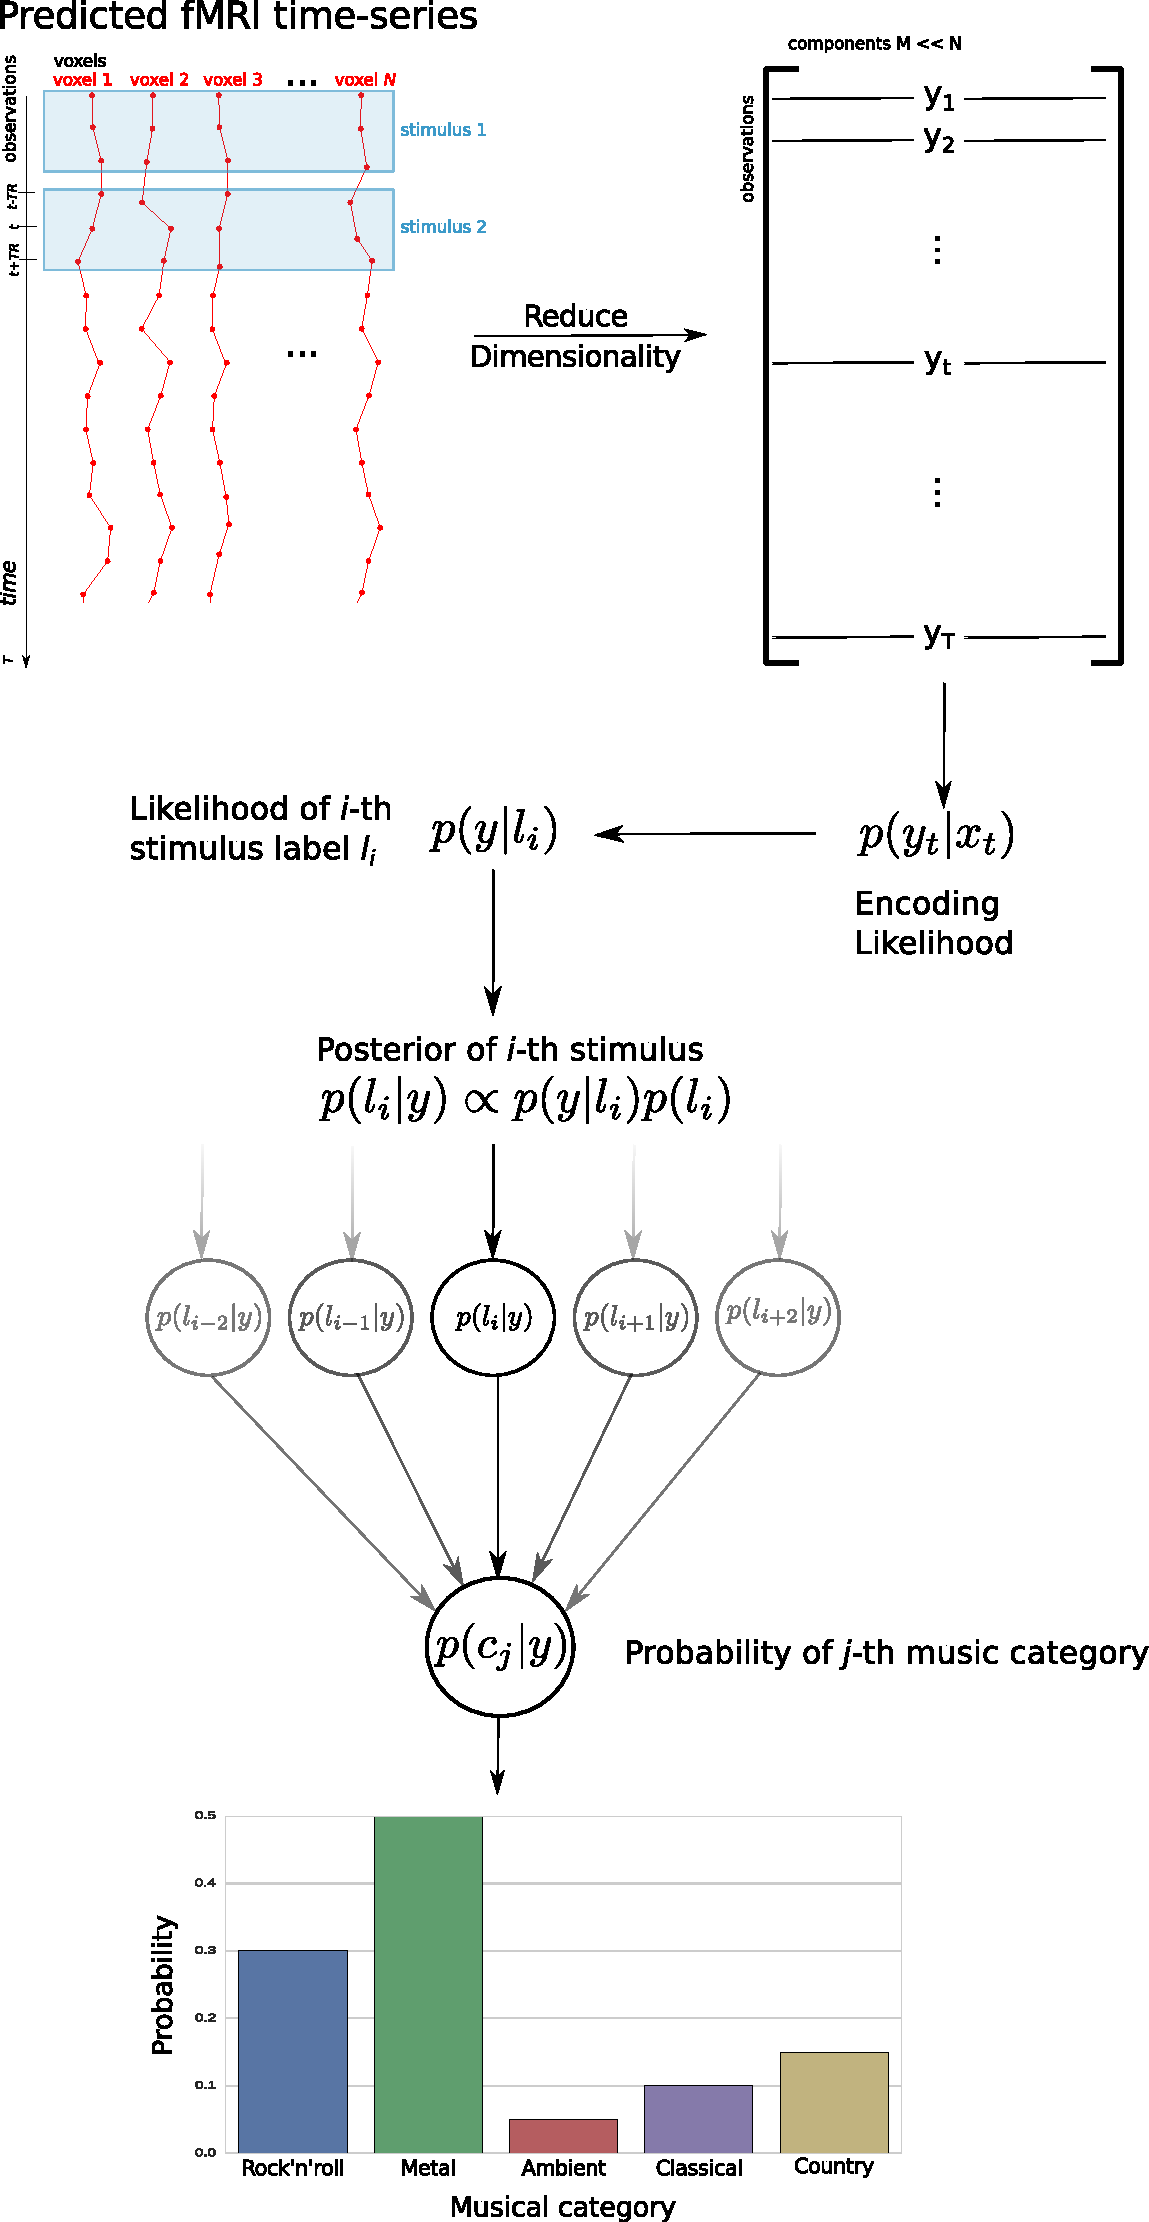
\includegraphics[width=.8\linewidth]{pics/decoding_scheme.pdf}

  \caption{A schematic overview of the decoding of music category. The
    predicted f{MRI} time series of the validation run is reduced in
    dimensionality by principal component analysis, and a multivariate-normal
    likelihood function $p(y_{t}|x_{t})$ is constructed.  From there, the
  probability distribution over music stimuli and subsequently musical
categories is estimated.}
%\todo[inline]{this is talking about a 2-part decoding scheme. would be good to
%  label those parts. Probably best to include a symbolic reference that the
%  basic scores (without decoding) are computed from the predicted time series
%  at the top. The manuscript is unclear how models from multiple voxels are
%treated in this case. Is the correlation distance computed for all timepoints
%of a stimulus across all the voxels? or per voxel and averaged?}


 \label{fig:decoding_scheme}
\end{figure}


\subsubsection*{Decoding}

Instead of testing the encoding performance, we can also test the performance
of a decoder based on the individual encoding models \citep{NG11} (Figure
\ref{fig:decoding_scheme}).

To go from the probability of a voxel activation
given stimulus features $p(y_{vt}|x_{t})$ to probability of stimulus features
given voxel activation $p(x_{t}|y_{t})$ we follow \citet{NG09} and separate our
decoding scheme into two parts. 

\paragraph{Single- to Multi-Voxel Encoding}

First we condense the large number of voxel-specific encoding models into one
multi-voxel encoding model.  To do this we project the predicted and observed
f{MRI} data onto the first $k$ principal components of the $[N\times V]$ matrix
of predicted BOLD activity. We choose $k$ via cross-validation to estimate the
number of principal components that maximize the decoding accuracy on the
training set for each participant.
As in \citet{NG09} we construct the $k$-dimensional multivariate normal
probability density function $p(y_{t}|x_{t})$ to obtain a likelihood function
across voxels. 

\paragraph{Multi-Voxel Encoding to Decoding}

We now express this likelihood in terms of the label of the music stimulus, instead of its LQ-MFS features.  We
use the simplifying assumption that the BOLD activity is influenced by the
music stimuli only through their LQ-MFS coefficients $x$, and --- given that
each music stimulus was associated with only three (lagged) LQ-MFS
representations --- the likelihood to observe a given triple of consecutive $y$
for a specific music stimulus $l_{i}$ is $p(y|l_{i}) \propto
p(y_{t-1}|x_{1})p(y_{t}|x_{2})p(y_{t+1}|x_{3})$ where $t$ is the sample 6
seconds after the start of the music stimulus and $x$ are the three LQ-MFS
feature vectors of this stimulus.  For a given triple of consecutive BOLD
activity $y$ from the same stimulus, we can now estimate the probability
distribution over music stimuli $p(l_{i}|y)$ (for $i=1..25$) by using Bayes'
rule: $p(l_{i}|y) \propto p(y|l_{i})p(l_{i})$.
Since each stimulus was presented was presented exactly once,
it has an uniform prior distribution with $p(l_{i})=\frac{1}{25}$. The mode of
this distribution is the most probable presented stimulus given the data. 
Additionally we can decode the musical genre of the presented stimulus given the observed
BOLD activity as the mode of $p(c_{i}|y) = \sum\nolimits_{l \in
  stim(c_{i})} p(l|y)$ where $stim(c_{i})$ are the labels of the stimuli
  belonging to the genre $c_{i}$. 


\subsection*{Voxel selection}

We varied the number of voxels used in the analysis, both for 3T and 7T
f{MRI} data, and selected which voxels to keep by two different criteria. Both
criteria were based on voxel characteristics in the training set only.

\paragraph{Selection by stability}

\citet{ML08} selected the 500 most stable voxels for their analysis. For a
single voxel, each run can be represented as a vector of BOLD activity, where
each entry is associated with one stimulus. A voxel's "stability score" is then
the average (pair-wise) correlation between the vectors of the eight runs for
all combinations of runs.  This criterion selects voxels with consistent
activation for each stimulus across runs.

\paragraph{Selection by $r^2$}

As we are interested in encoding performance, we can use the quality of
predictions of each voxel's encoding model as a selection criterion. We compute
the coefficient of determination $r^2$ for each voxel-specific encoding model
in the training set. Using this criterion selects voxels whose activity can be
explained best by an LQ-MFS-based encoding model.

\section*{Results}

We trained voxel-wise encoding models to predict voxel activity using a LQ-MFS
representation of music stimuli in 3T and 7T f{MRI} data.
First, we evaluate each voxel's encoding model individually.
Figure \ref{fig:r2_plot} shows $r2$ values from an eight fold cross-validation
of the 10000 voxels with highest $r2$ averaged across participants.
While voxel-wise encoding models in 3T perform similarly or even better than 7T
in the best predicted voxels, voxel-wise encoding models in 7T clearly
outperform models in 3T in all other voxels.

\begin{figure}
  \centering
  \includegraphics[width=\linewidth]{pics/r2_plot.pdf}
	
  \caption{Average $r2$ across participants and 95\% confidence interval for the 10000 voxels with
    highest $r2$, sorted by $r2$, for 3T and 7T.
  }

 \label{fig:r2_plot}\end{figure}

Next, we evaluate sets of voxel-wise encoding models for 3T and 7T using several
quality metrics.
We varied the number of voxels used in the analysis and how they were selected,
both for 3T and 7T f{MRI} data, and compared the resulting differences in
three quality metrics of encoding models.
To differentiate between effects of voxel number and overall volume of the voxels,
which differs in 3T and 7T, we show the results as a function of the number of voxels,
as well as overall volume of these voxels.

\begin{figure*}
  \centering
  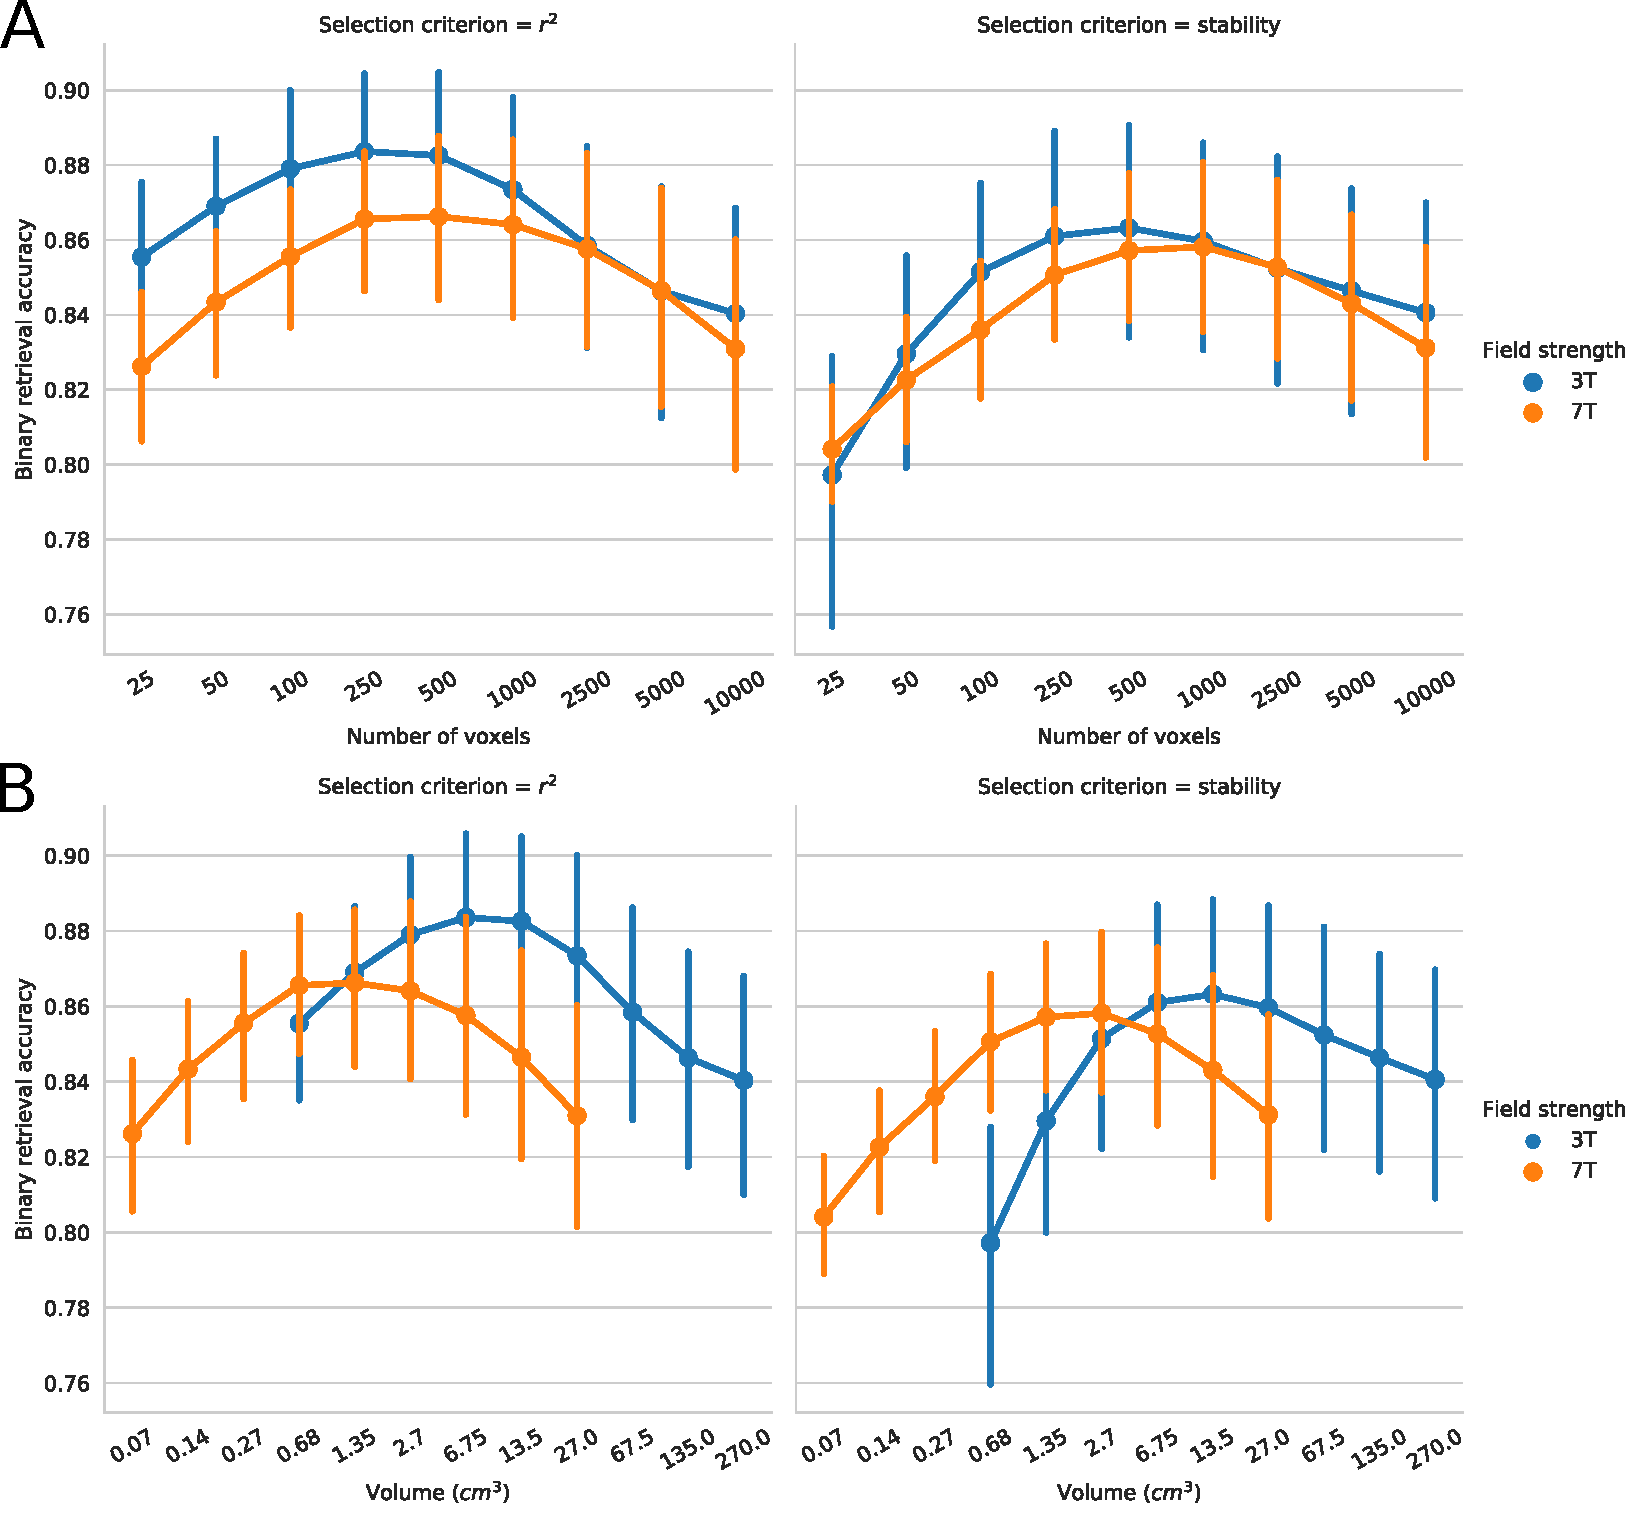
\includegraphics[width=\linewidth]{pics/binary.pdf}
	
  \caption{\textbf{A} Mean binary retrieval accuracy as a function of the
  included number of voxels for 3T and 7T, for stability- and $r^2$-based
  voxel selection. Error bars denote the bootstrapped 95\% confidence interval
  of the mean. The mean is taken over binary retrieval accuracies of eight runs
  for each of the 19 participants. \textbf{B} Mean binary retrieval accuracy as
a function of the overall volume of the included voxels for 3T and 7T, for
stability- and $r^2$-based voxel selection.
}

 \label{fig:binary_retrieval}\end{figure*}

\subsection*{Binary retrieval accuracy}

Figure \ref{fig:binary_retrieval} shows differences in binary retrieval accuracy
for different numbers of voxels, selection strategies, and field strength.
%TODO: indicate maxima?
For both 3T and 7T data, and both selection strategies, the maximum binary
retrieval accuracy is achieved with relatively low number of voxels (3T and
$r2$: 250 voxels, 7T and $r2$: 500 voxels, 3T and stability selection: 500
voxels, 7T and stability selection: 1000 voxels) and decreases the more voxels are
included.
For both stability selection criteria, 3T outperforms or is equal to 7T across
all numbers of voxels.
With regard to the voxel selection strategies, selection by $r2$ outperforms or
is equal to selection by stability across all numbers of voxels (Figure
\ref{fig:binary_retrieval_selection}).

\begin{figure*}
  \centering
    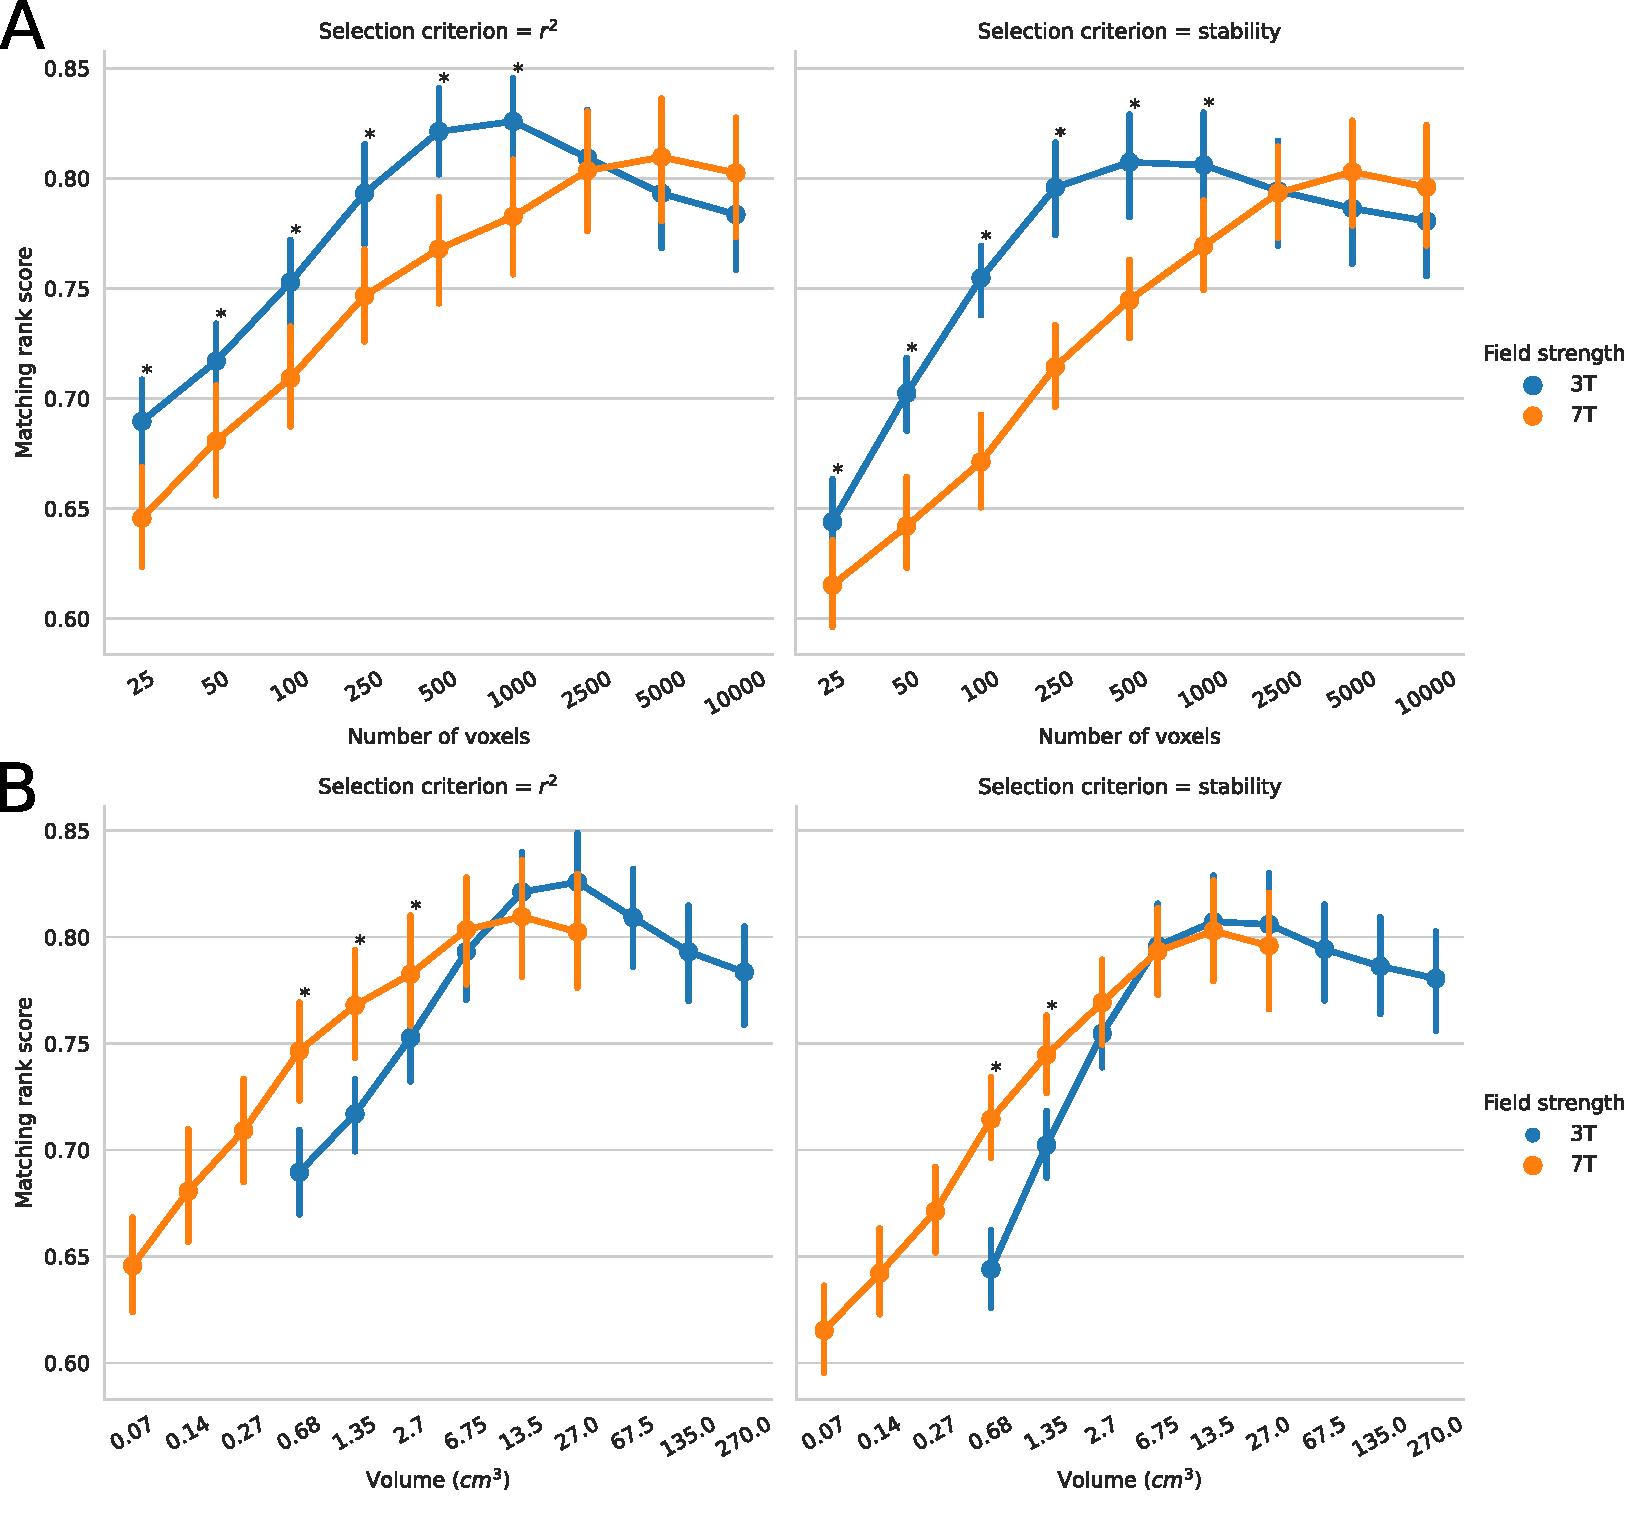
\includegraphics[width=\linewidth]{pics/rank.pdf}
	
  \caption{\textbf{A} Mean matching rank score as a function of the included number
  of voxels for 3T and 7T, for stability- and $r^2$-based voxel selection.
  Error bars denote the bootstrapped 95\% confidence interval of the mean. The
  mean is taken over binary retrieval accuracies of eight runs for each of the
  19 participants. \textbf{B} Mean matching rank score as a function of the overall
volume of the included voxels for 3T and 7T, for stability- and
$r^2$-based voxel selection.}

 \label{fig:matching_score}
\end{figure*}

\subsection*{Matching score}

Figure \ref{fig:matching_score} shows differences in matching score
for different numbers of voxels, selection strategies, and field strength.
Matching scores in both 3T and 7T data peak at high numbers of voxels (3T and
$r2$: 1000 voxels, 7T and $r2$: 5000 voxels, 3T and stability selection: 500
voxels, 7T and stability selection: 5000 voxels).
Indexing by the overall volumes these voxels encompass reveals that the matching
score peaks for 3T and 7T at (for stability selection) or close to (for
selection by $r2$) the same volume.
For both stability selection and selection by $r2$, 3T outperforms 7T for the
same number of voxels, except for the largest two numbers of voxels, and --- in
terms of the volume the voxels take --- 7T outperforms 3T for volumes up to 2.7
$cm^{3}$ and 3T outperforms 7T for volumes beyond 27 $cm^{3}$.
Furthermore, for 3T data, selection by stability and selection by $r2$ perform
similarly, while selection by $r2$ outperforms selection by stability
consistently in 7T data (Figure \ref{fig:matching_score_selection}).

\begin{figure*}
  \centering
    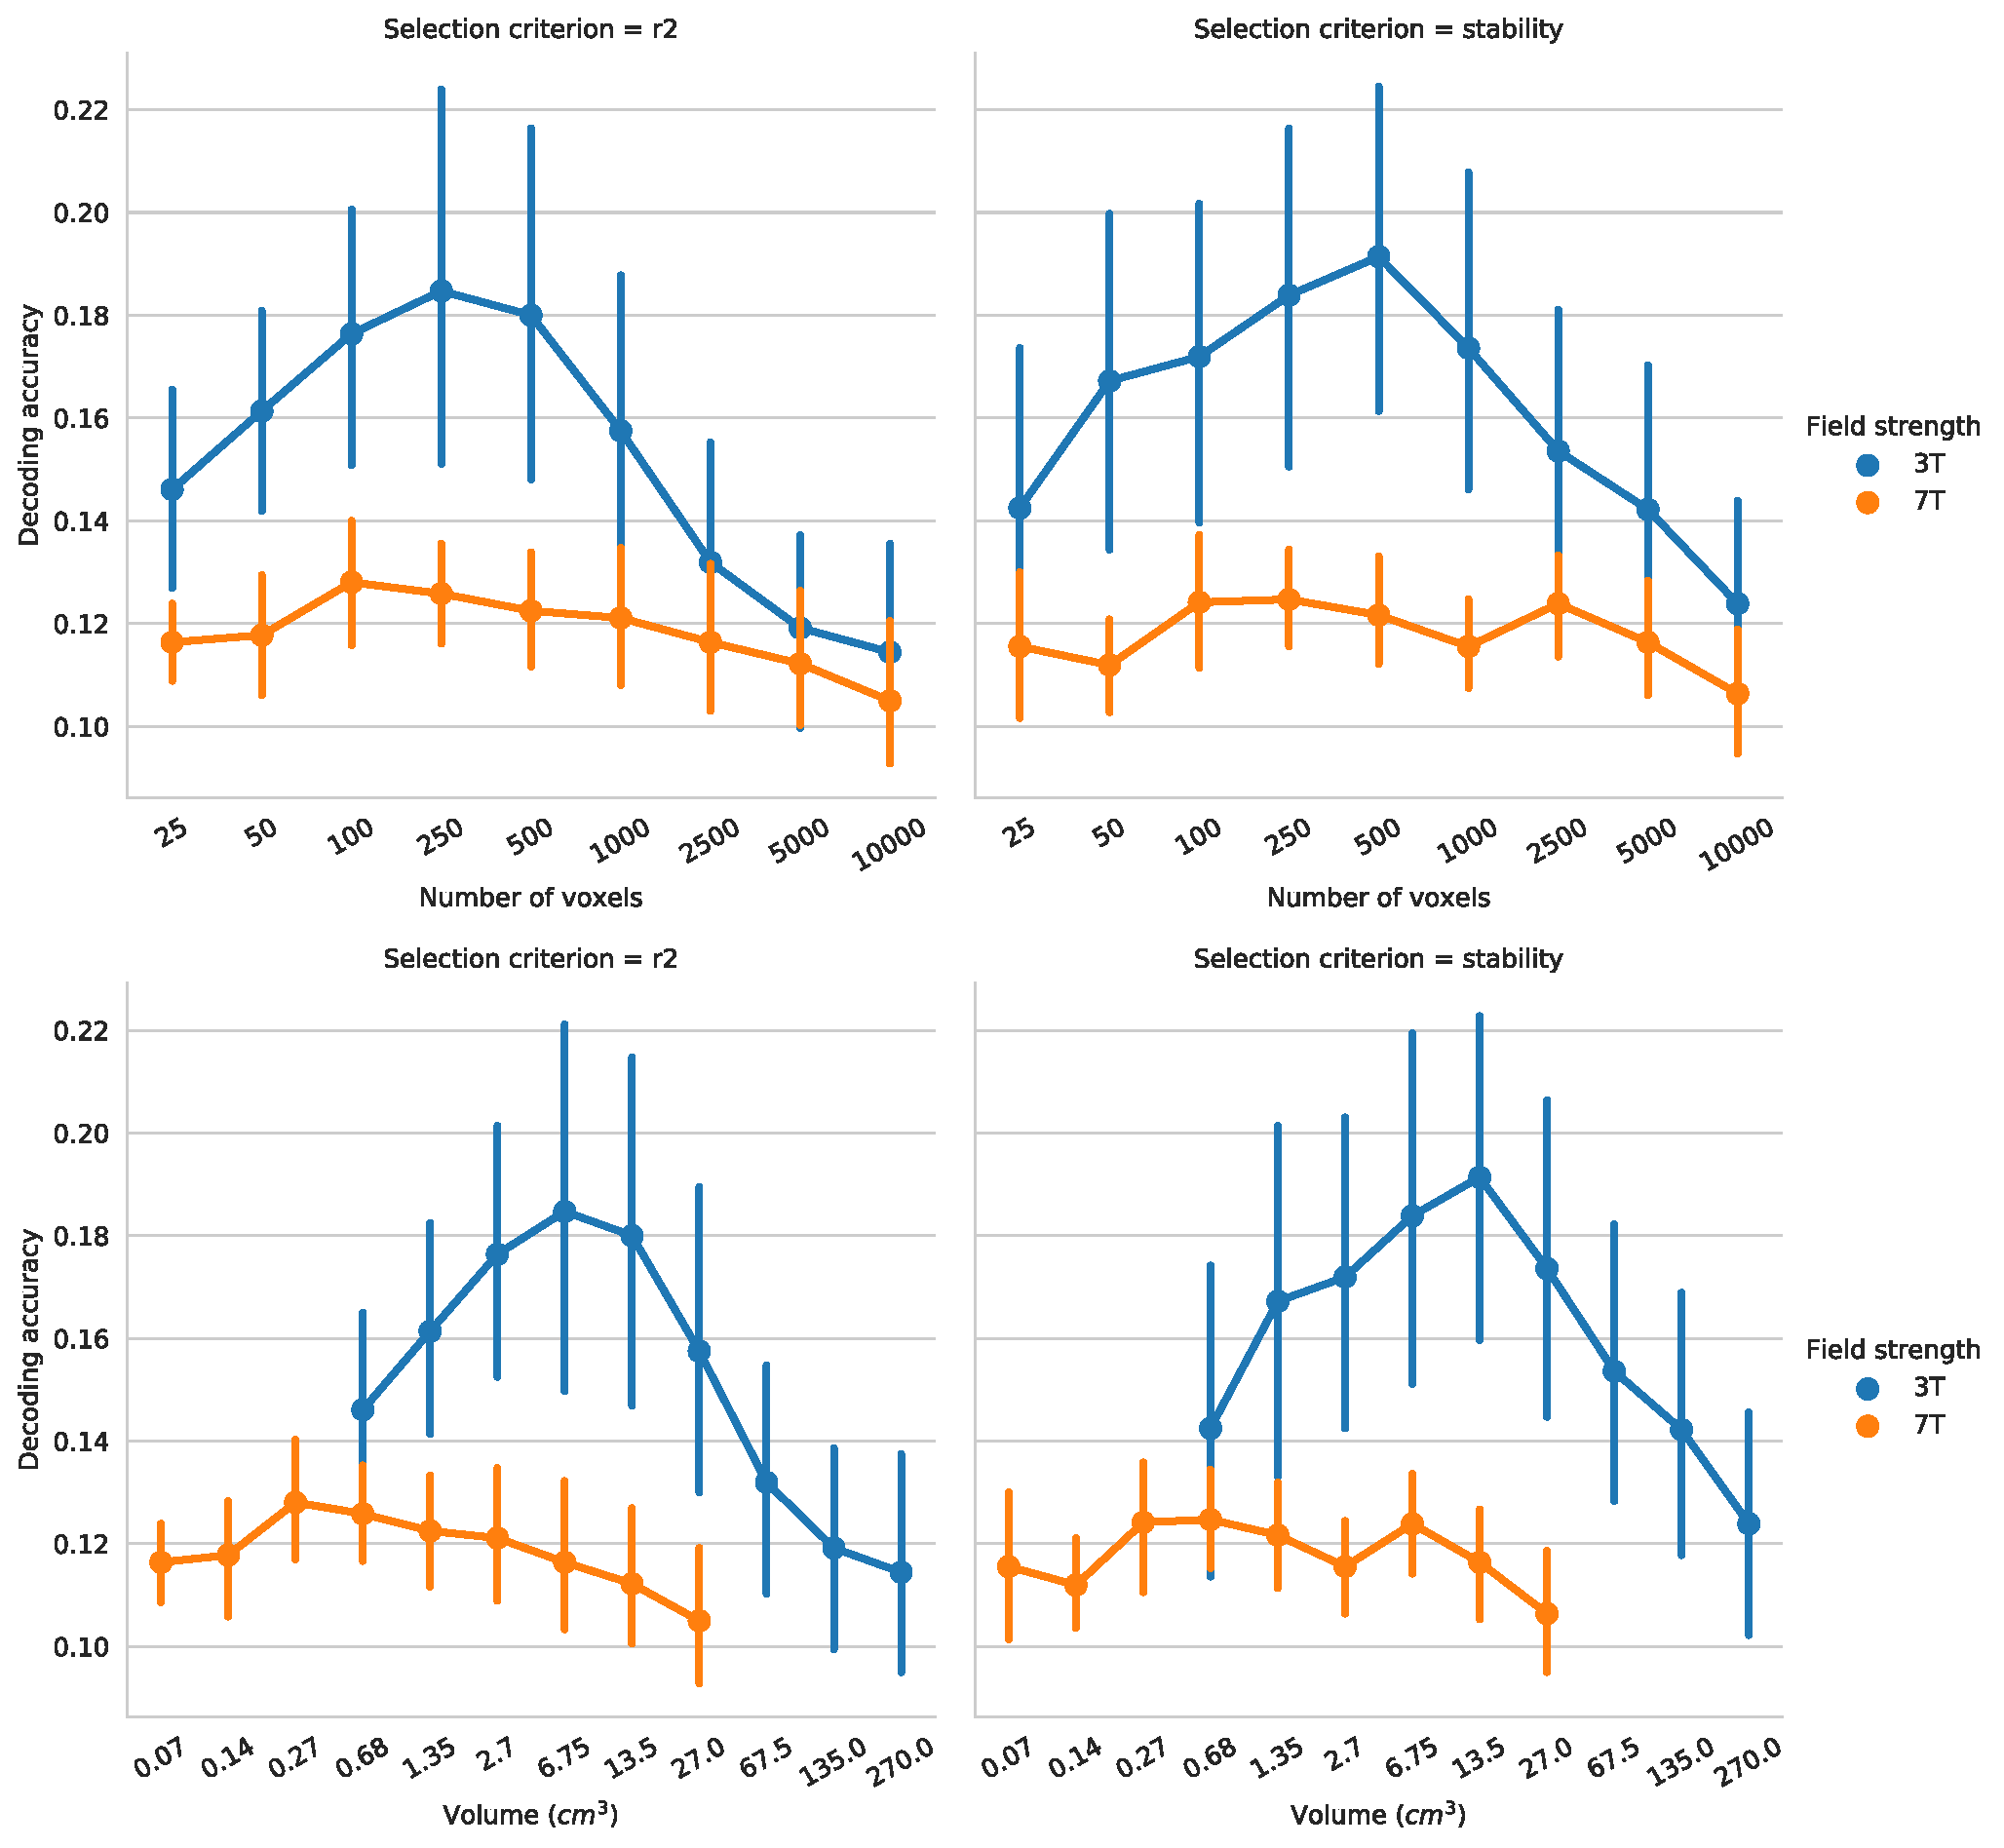
\includegraphics[width=\linewidth]{pics/decoding.pdf}

	\caption{\textbf{A} Mean decoding accuracy of individual music stimuli as a function of
  the included number of voxels for 3T and 7T, for stability- and
  $r^2$-based voxel selection. Error bars denote the bootstrapped 95\%
  confidence interval of the mean. The mean is taken over decoding
  accuracies of eight runs for each of the 19 participants. Chance level is
    0.04. \textbf{B} Mean
decoding accuracy of individual music stimuli as a function of the overall volume of the
included voxels for 3T and 7T, for stability- and $r^2$-based voxel
selection. Chance level is 0.04.
}
 \label{fig:decoding_accuracy_stimulus}
\end{figure*}

\begin{figure*}
  \centering
  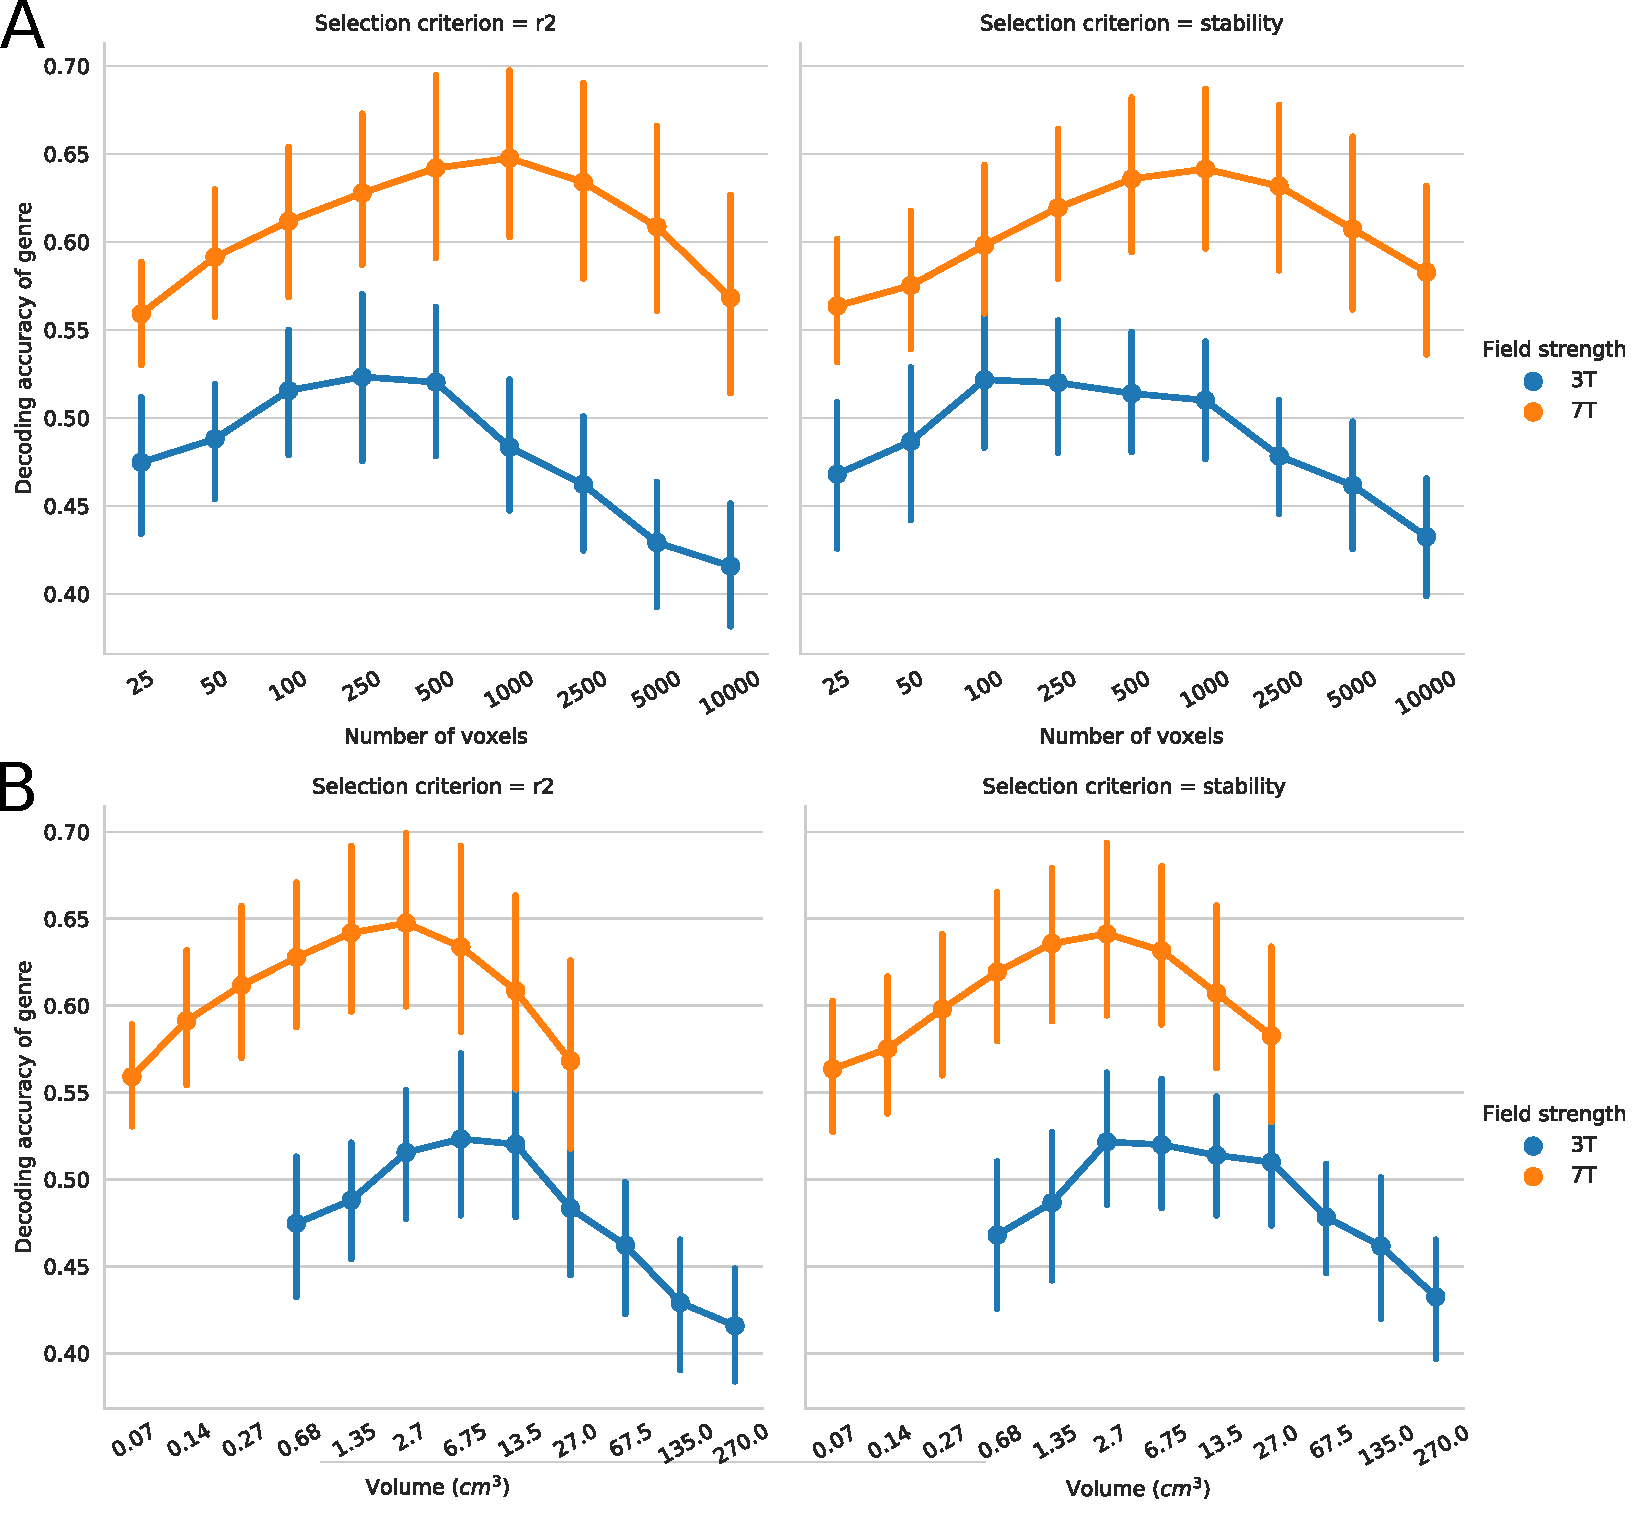
\includegraphics[width=\linewidth]{pics/decoding_genre.pdf}

  \caption{\textbf{A} Mean decoding accuracy of music category as a function of
  the included number of voxels for 3T and 7T, for stability- and
  $r^2$-based voxel selection. Error bars denote the bootstrapped 95\%
  confidence interval of the mean. The mean is taken over decoding
  accuracies of eight runs for each of the 19 participants. \textbf{B} Mean
decoding accuracy of music category as a function of the overall volume of the
included voxels for 3T and 7T, for stability- and $r^2$-based voxel
selection.
}

 \label{fig:decoding_accuracy}
\end{figure*}

\begin{figure}
  \centering
  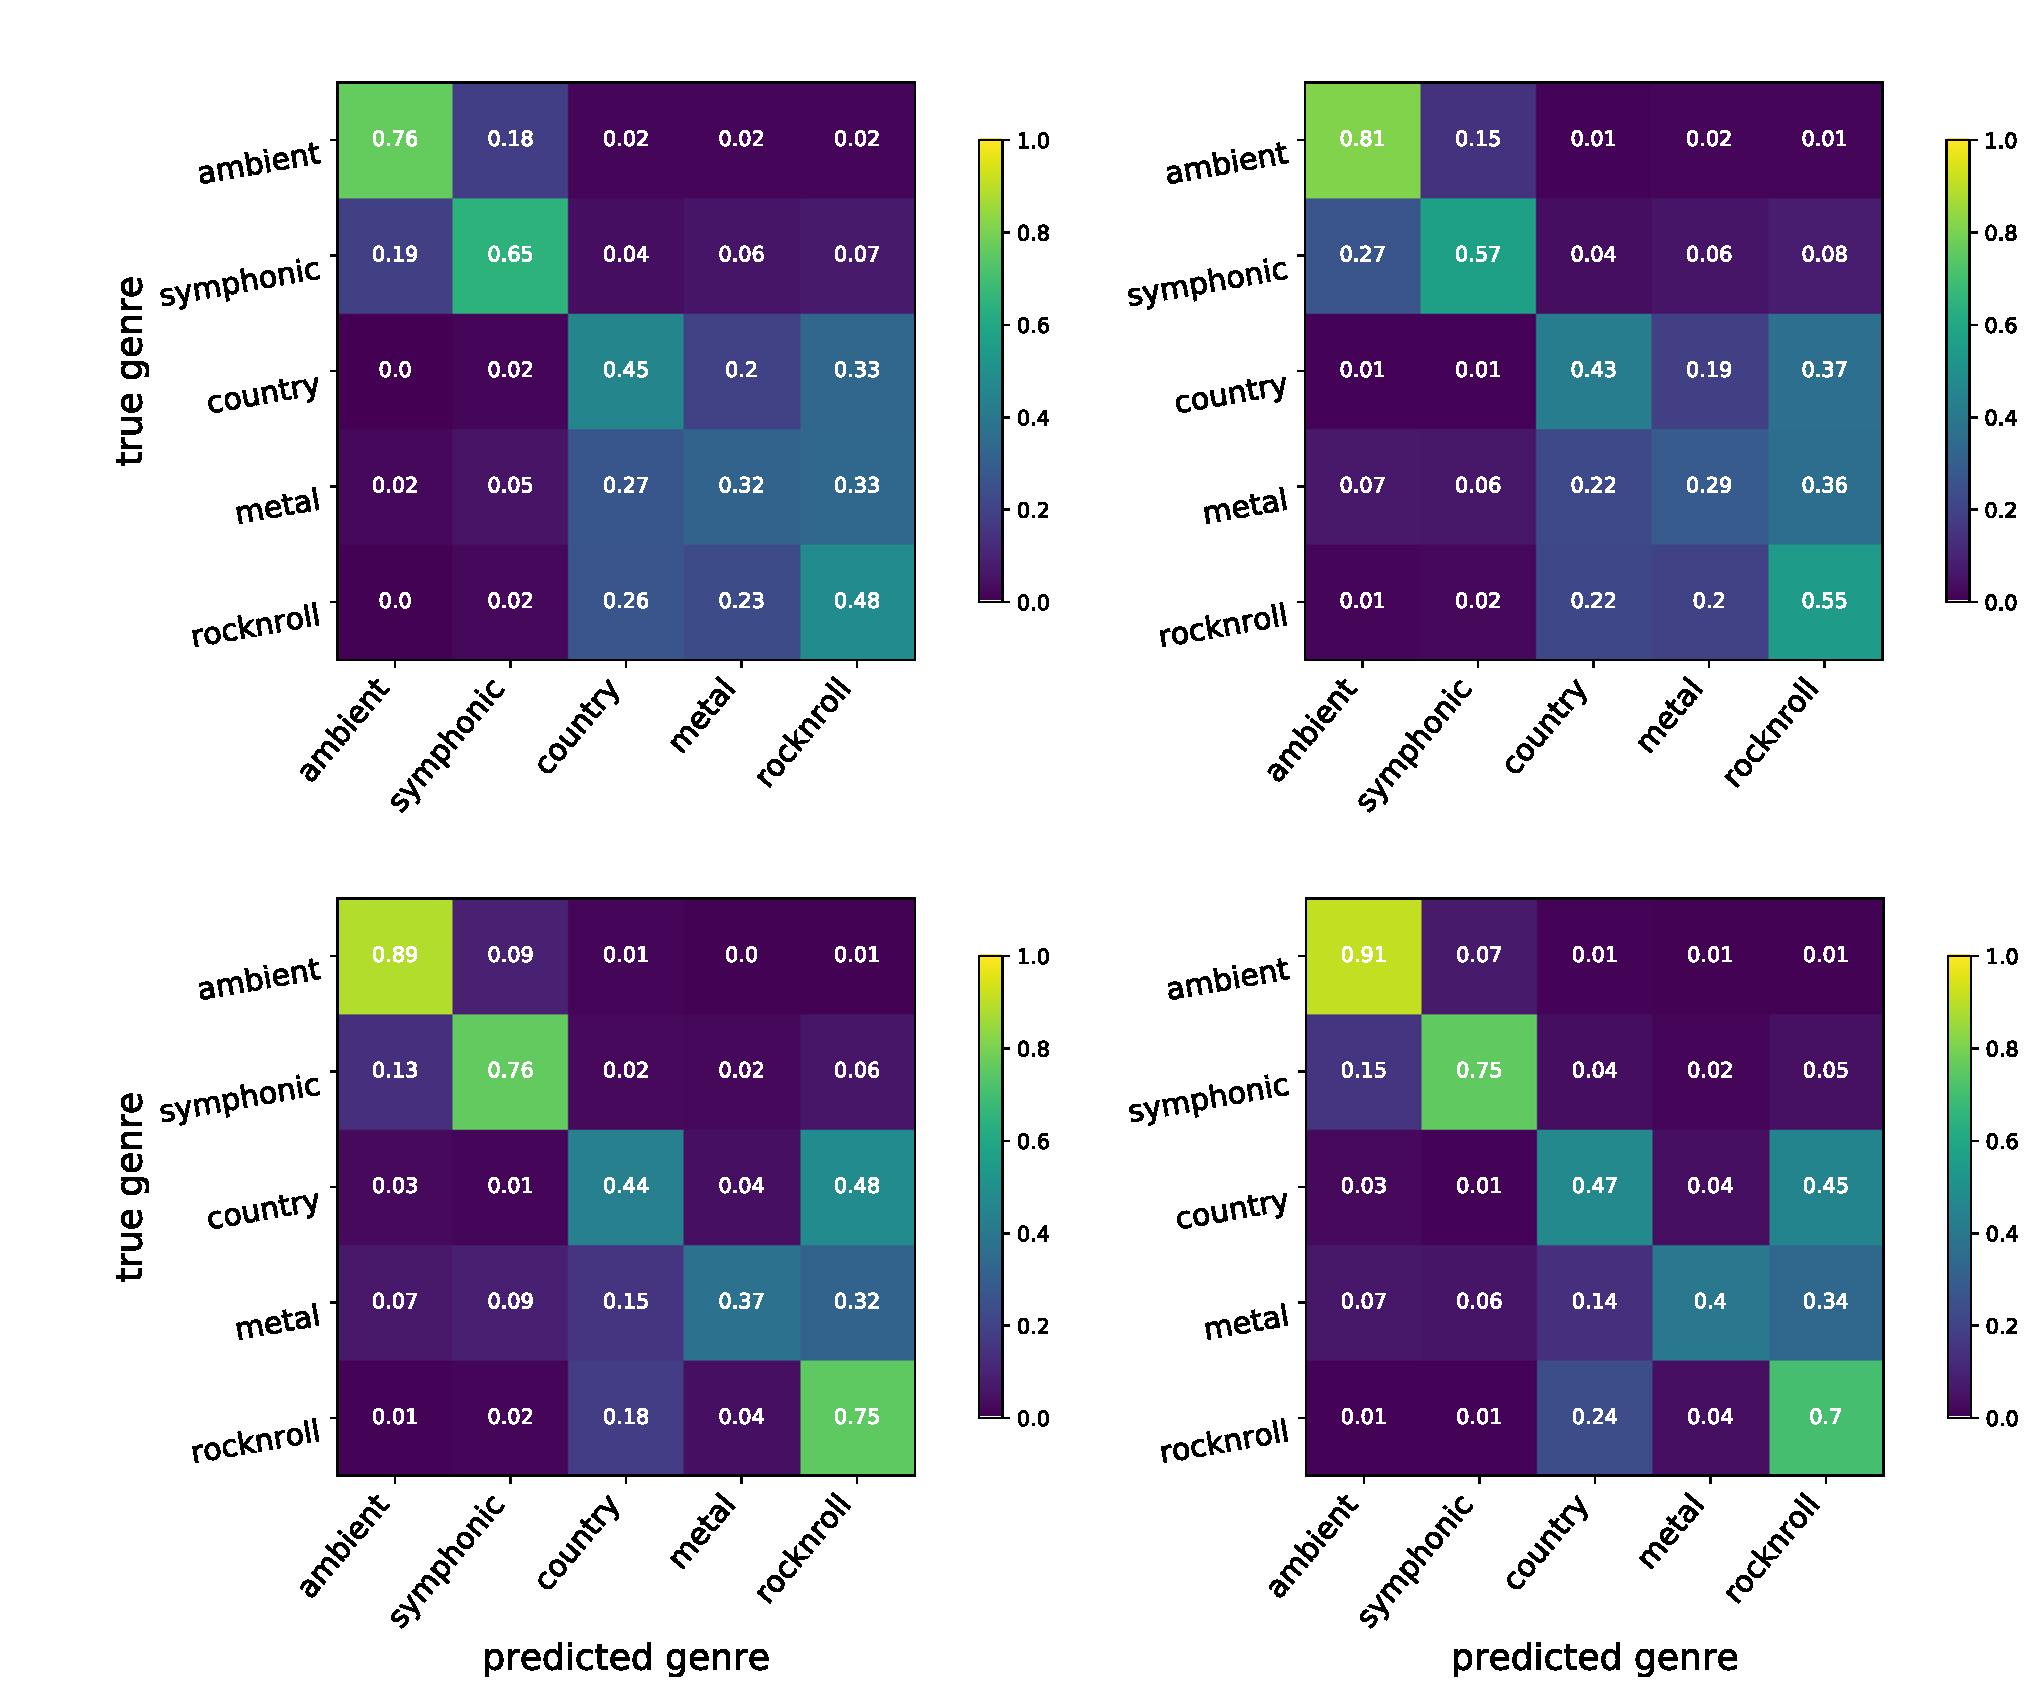
\includegraphics[width=\linewidth]{pics/conf_mats.pdf}

  \caption{ Confusion matrices for genre decoding, separated by field-strength and voxel selection. Each confusion matrix is averaged across the different number of voxels, participants and runs.}

 \label{fig:confusion_matrices}
\end{figure}

\subsection*{Decoding accuracy}

Figure \ref{fig:decoding_accuracy_stimulus} shows the accuracy of decoding each
individual stimulus (chance level 0.04) for different numbers of voxels,
selection strategies, and field strength.
A large discrepancy between the decoding performance of individual stimuli in 3T
and 7T is visible: if voxels are selected by stability, 3T outperforms 7T for
all numbers of voxels, if voxels are selected by $r2$, 3T outperforms 7T for all
but the two highest numbers of voxels.
For 7T data, the number of voxels matters little, however, for 3T data, optimal
decoding accuracy is reached at a relatively low number of voxels (250 voxels
for selection by $r2$ and selection by stability), and subsequently decreases if
more voxels are included.
However, decoding accuracy in 3T shows large variability, making comparisons
between different numbers of voxels difficult.

Instead of decoding individual stimuli, we can also decode the musical genre of
each individual stimulus.
Figure \ref{fig:decoding_accuracy} shows the accuracy of decoding music genre
(chance level 0.20) for different numbers of voxels, selection strategies,
and field strength.
Here a different pattern emerges: decoding accuracy is higher for 7T data than for
3T data, across all numbers of voxels and selection criteria.
For both selection strategies, 7T shows higher genre decoding accuracy for high
numbers of voxels, while 3T shows higher genre decoding accuracy for lower
numbers of voxels.

We next want to answer the question which musical genres can be best predicted,
and if those differ between 3T and 7T data.
For this we compute the confusion matrix from the out-of-sample predictions of
all classifiers: Rows denote the stimulus' true genre, columns denote the
predicted genre. Each cell contains the count -- or proportion
-- of occurences of this combination of true and predicted genres.
Maximum classification accuracy leads to a diagonal confusion matrix.

Figure \ref{fig:confusion_matrices} shows the confusion matrices averaged across
numbers of voxels for different field strength and selection criteria.

The occurences are normalized per row, and their mean proportion across numbers
of voxels are indicated in each cell. All confusion matrices show a higher
misclassification between genres that contain speech (country, rock'n'roll and heavy metal)
and between instrumental genres (ambient and symphonic), while very few genres that contain speech are
incorrectly classified as instrumental or vice versa.
The increased genre decoding accuracy in 7T is thus due to a better
discrimination between the two instrumental genres --- ambient and symphonic ---
and between the three vocal genres --- country, rock'n'roll, and heavy metal.

%\begin{figure}
%  \centering
%  \def\svgwidth{\linewidth}
%  \input{pics/r2_means.pdf_tex}
%	
%  \caption{ Mean $r^2$ of voxels sorted by $r^2$.}
%
% \label{fig:r2}
%\end{figure}
%
%\begin{figure}
%  \centering
%  \def\svgwidth{\linewidth}
%  \input{pics/Mean_fstatistic_stim_cat.pdf_tex}
%	
%  \caption{ Mean voxel-wise F-statistic for the f{MRI} time series averaged over
%  the voxels selected by $r^2$ for genre or stimulus.}
%
% \label{fig:anova}
%\end{figure}
%
%\begin{figure}
%  \centering
%  \def\svgwidth{\linewidth}
%  \input{pics/Mean_fstatistic_stim_cat_yhat.pdf_tex}
%	
%  \caption{ Mean voxel-wise F-statistic for the predicted f{MRI} time series averaged over
%  the voxels selected by $r^2$ for genre or stimulus.}
%
% \label{fig:anova_yhat}
%\end{figure}
%
\section*{Discussion}

Our results show all three quality metrics varying with the number of
voxels and voxel selection strategies in both low and high field strengths.
We demonstrate that the patterns of this variation differ between validation strategies
and that field strength, voxel selection, and voxel number all affect these metrics
differently.

However, in spite of these inconsistencies, some common patterns emerge:
voxel-wise encoding models in 3T f{MRI} data outperform voxel-wise encoding models in
7T f{MRI} data in all but one quality metric.
This indicates that high field strength does not provide more information per
se, since stimuli can't be differentiated better in general, in spite of the higher
$r2$ in individual voxels in 7T than in 3T.
Only when a decoding framework incorporates the relevant information, in our
case the musical genre, can it harness the improved signal-to-noise ratio of
higher field strength.
Our result thus constrasts a  previous study \citep{SF14} that found a better
performance for 7T data for the matching score, although using a different
number of stimuli in the 3T and 7T datasets.

One reason for this, could be that training encoding models on stimulus features
can make stimulus labels somewhat arbitrary.
Two stimuli might be quite similar, and the encoding model might correctly translate this into similar
predicted BOLD activity, and hence a higher $r2$,  yet this similarity could decrease a quality measure
that is based on the correct discrimination between individual stimuli.

We observe another common pattern in the effect of voxel selection strategy:
selecting the voxels by $r^2$ either improves upon or performs indistinguishably
from selection by a stability criterion.
One reason that this effect is especially prominent when only few voxels are included could
be the quickly diminishing returns for higher number of voxels: voxels in which 
an encoding model performs well are already included, and each additional voxel
decreases the joint encoding performance.

Interestingly, this pattern is not seen in the
matching score, where performance in 7T is worse for the smallest number
of voxels and continually increases when more voxels are included.
In fact, this holds true for selection by both $r2$ and a stability criterion,
and thus differentiates the matching score from both binary retrieval accuracy,
as well as decoding accuracy.

Accordingly, indexing by the overall volume of the selected voxels,
instead of their number, reveals similarities in performance when 3T
and 7T encoding models are trained on a similar volume in the matching
score, yet all other metrics show a higher sensitivity to the number of
voxels.

To conclude, we can abstract several recommendations for applying and validating
voxel-wise encoding models.

%r2 > stability selection
First, it is likely that selecting voxels by the quality of its encoding model,
such as the $r2$ score, will outperform a selection of voxels based on their
stable response to the stimulus --- however, this difference diminishes for
large numbers of voxels.

%number of voxels matters: to compare two encoding models one has to control for
%it
Second, the number of voxels used has a large effect on all quality metrics, and
to compare two sets of voxel-wise encoding models even on the same stimuli, one
has to control for them.
For most quality metrics, this control is most easily exercised by fixing the
number of voxels directly, however, in case of the matching score, it can be
more meaningful to fix the overall volume the two sets of encoding models
encompass.
%For most applications of voxel-wise encoding models, this distinction will not
%matter, since comparisons between encoding models rarely encompass different
%voxel sizes, however, to judge the difference in performance for

Third, while higher field strength might lead to better individual encoding
models, it might not improve their decoding accuracy.
The key insight is, that higher field strength can decrease the decoding
accuracy for some labels of the stimulus, i.e. the decoding of individual
stimuli, yet increase the decoding accuracy for other labels, i.e the decoding
of the musical genre of individual stimuli.
Thus, one has to exercise caution, when choosing which label to decode from a set
of encoding models.

However, to assess if these recommendations generalize, more data are
needed, since the results in this study are based on only two f{MRI} datasets
encompassing the same auditory stimuli recorded in 3- and 7T.
This facilitates a comparison between different field
strengths, yet, further work is needed to show that these conclusions hold beyond
this set of stimuli, our chosen stimulus representation, and even beyond the auditory domain.

Nonetheless, this work shows the significance of on an often under-appreciated aspect of
computational models in neuroimaging: arbitrary choices in the data analysis,
-- like the number of voxels used or how they are selected --
have a considerable impact on the performance evaluation of
voxel-wise encoding models. Furthermore, the impact of these parameters is
highly inconsistent across the considered validation strategies.
The effects of these parameters are rarely known a-priori, and each choice of a specific value can often
be easily justified, yet this undisclosed flexibility leads to considerable researcher degrees-of-freedom
\citep{SNS11,hong2019false} and will bias the comparison between different
voxel-wise encoding models.

\section*{Author contributions}
%In order to give appropriate credit to each author of an article, the
%individual contributions of each author to the manuscript should be detailed
%in this section. We recommend using author initials and then stating briefly
%how they contributed.

MB performed the analysis and wrote the manuscript.
JSG contributed to the manuscript.
MH contributed to the manuscript.
\todo{some authors are missing here}


\section*{Competing Interests}

No competing interests were disclosed.

\section*{Grant Information}

This research was, in part, supported by the German Federal Ministry of
Education and Research (BMBF) as part of a US-German collaboration in
computational neuroscience (CRCNS; awarded to James Haxby, Peter Ramadge, and
Michael Hanke), co-funded by the BMBF and the US National Science Foundation
(BMBF 01GQ1112; NSF 1129855).  Work on the data-sharing technology employed for
this research was supported by US-German CRCNS project awarded to
Yaroslav~O.~Halchenko and Michael~Hanke, co-funded by the BMBF and the US
National Science Foundation (BMBF 01GQ1411; NSF 1429999).  Michael Hanke was
supported by funds from the German federal state of Saxony-Anhalt, Project:
Center for Behavioral Brain Sciences.


\section*{Acknowledgements}
%This section should acknowledge anyone who contributed to the research or the
%article but who does not qualify as an author based on the criteria provided
%earlier (e.g. someone or an organisation that provided writing assistance).
%Please state how they contributed; authors should obtain permission to
%acknowledge from all those mentioned in the Acknowledgements section.  Please
%do not list grant funding in this section (this should be included in the
%Grant information section - See above).

We are grateful to Michael Casey and the musicians ;) \ldots

\todo[inline]{express gratitude}

\bibliography{references}

\beginsupplement
\section*{Supplementary information} \label{supplemental}
\begin{figure}
  \centering
  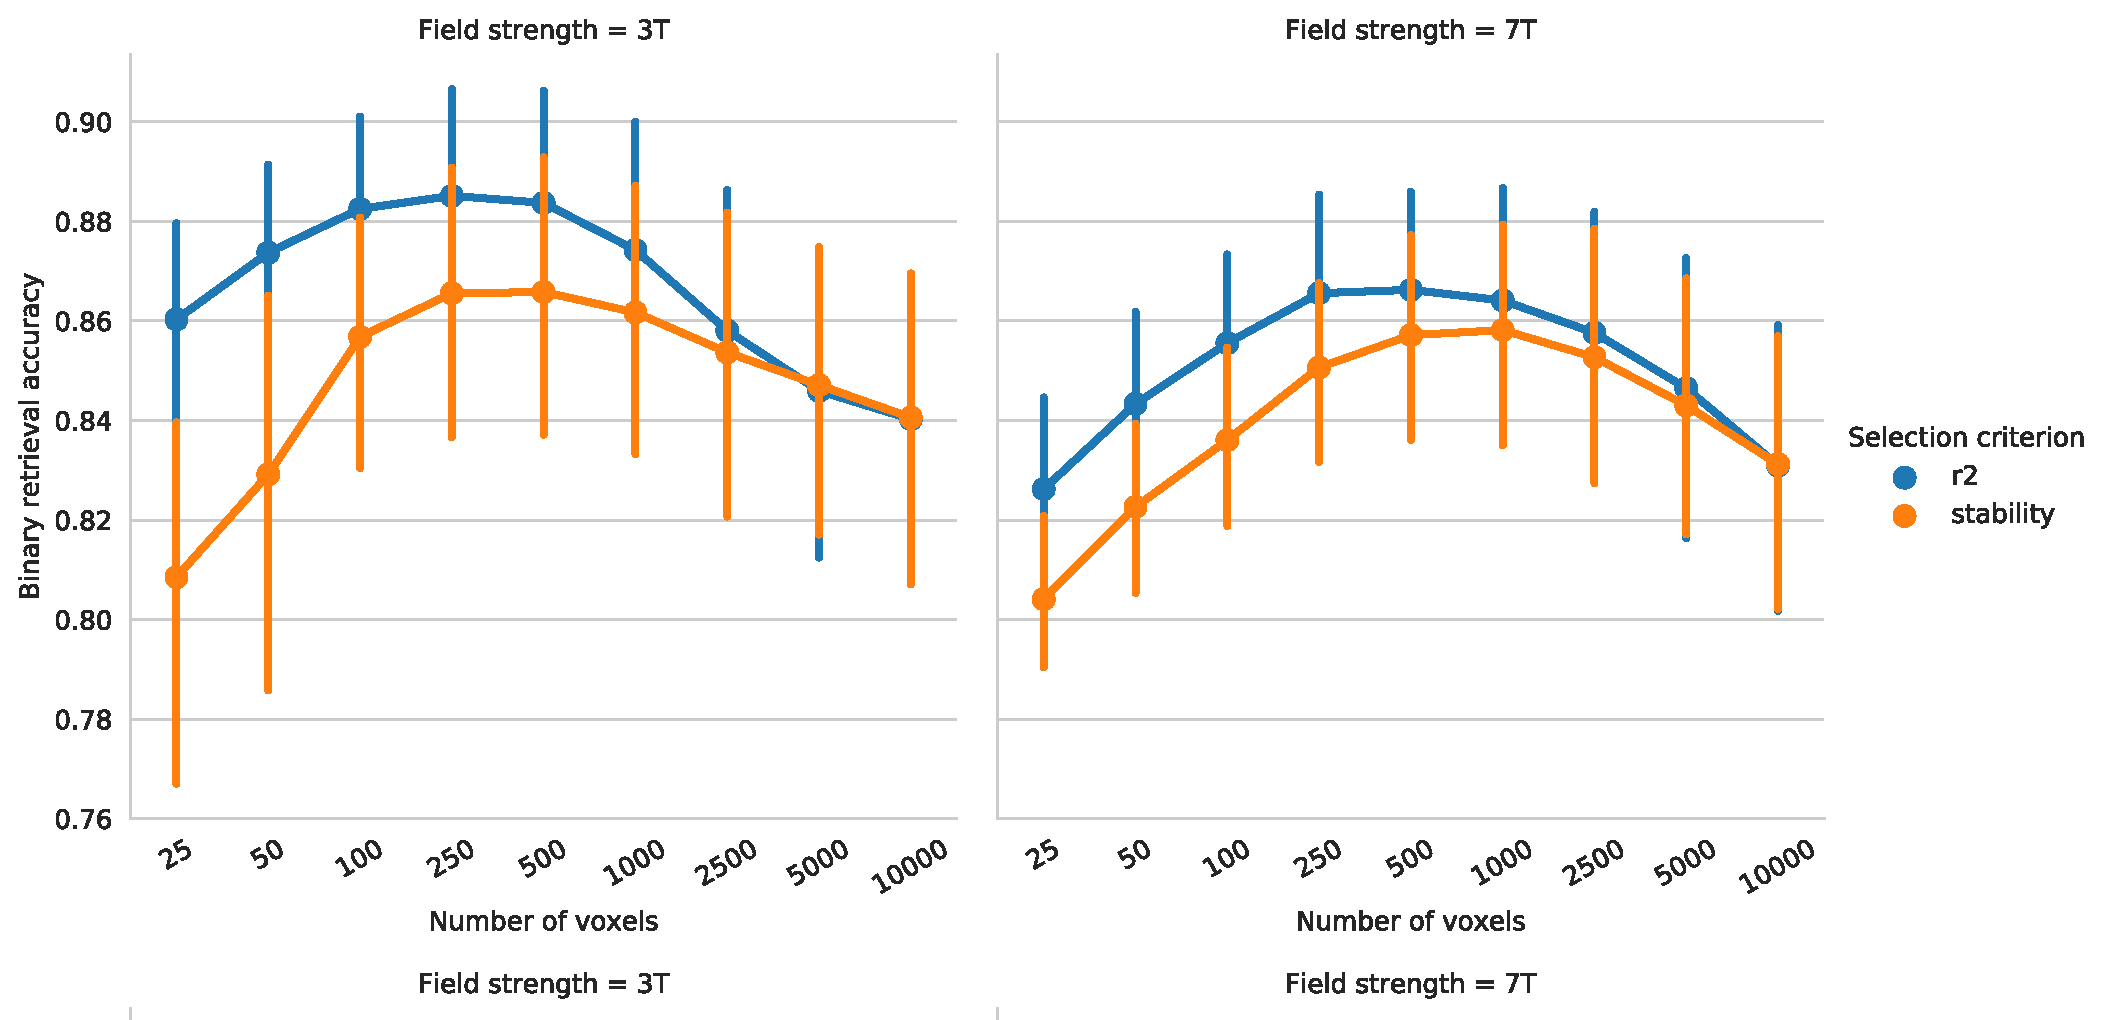
\includegraphics[width=\linewidth]{pics/binary_selection.pdf}
	
  \caption{\textbf{A} Mean binary retrieval accuracy as a function of the
  included number of voxels for 3T and 7T, for stability- and $r^2$-based
  voxel selection. Error bars denote the bootstrapped 95\% confidence interval
  of the mean. The mean is taken over binary retrieval accuracies of eight runs
  for each of the 19 participants. \textbf{B} Mean binary retrieval accuracy as
a function of the overall volume of the included voxels for 3T and 7T, for
stability- and $r^2$-based voxel selection.
}

 \label{fig:binary_retrieval_selection}\end{figure}

\begin{figure}
  \centering
    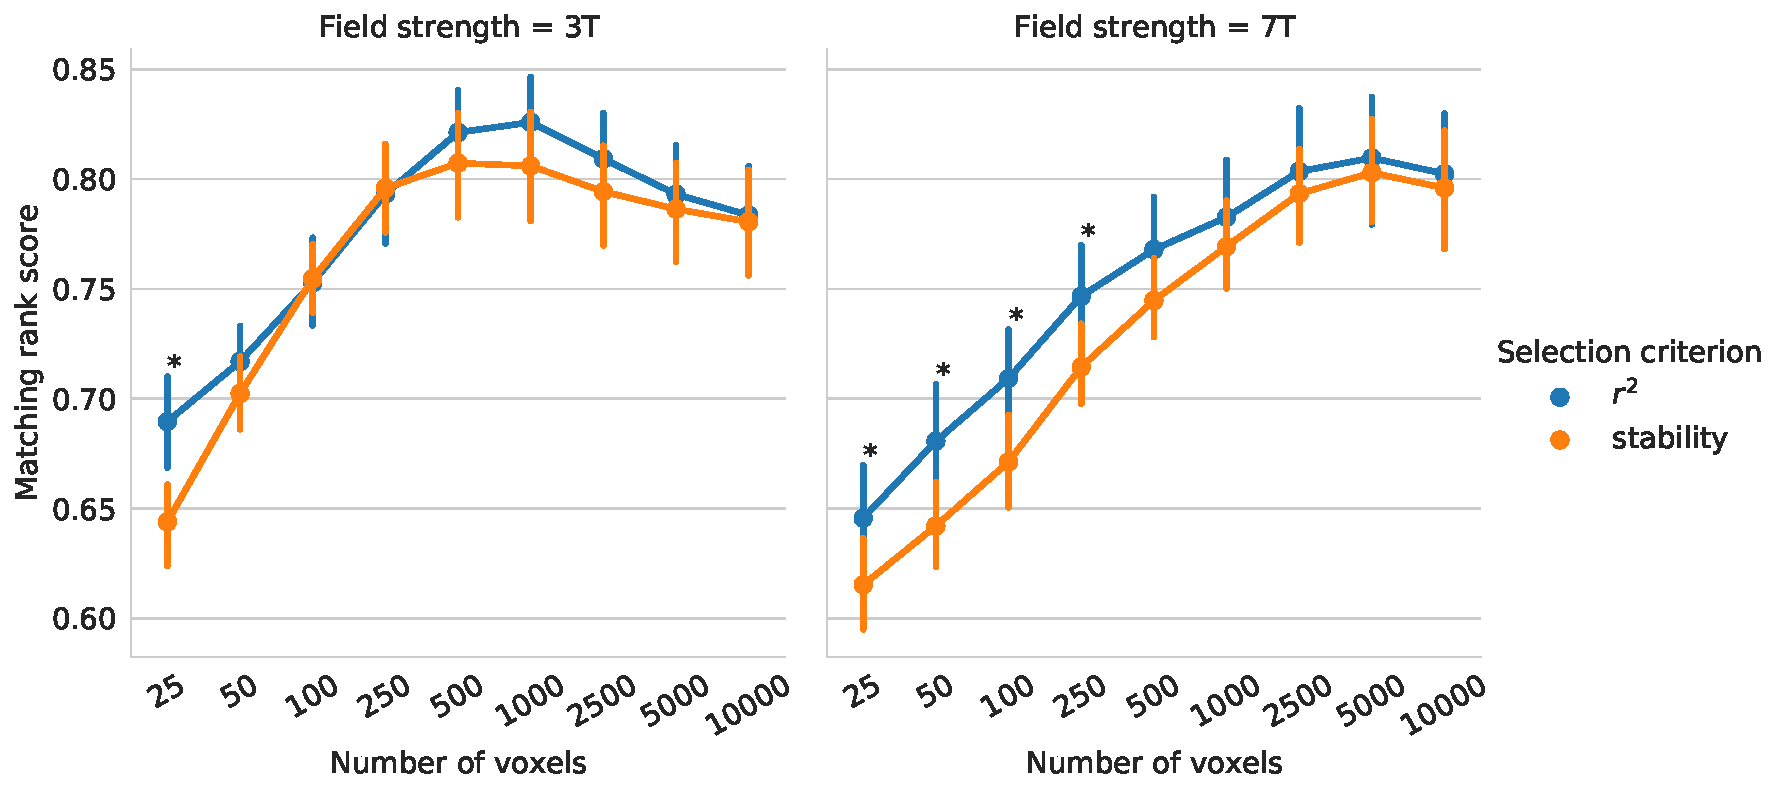
\includegraphics[width=\linewidth]{pics/rank_selection.pdf}
	
  \caption{\textbf{A} Mean matching rank score as a function of the included number
  of voxels for 3T and 7T, for stability- and $r^2$-based voxel selection.
  Error bars denote the bootstrapped 95\% confidence interval of the mean. The
  mean is taken over binary retrieval accuracies of eight runs for each of the
  19 participants. \textbf{B} Mean matching rank score as a function of the overall
volume of the included voxels for 3T and 7T, for stability- and
$r^2$-based voxel selection.}

 \label{fig:matching_score_selection}
\end{figure}


\begin{figure}
  \centering
    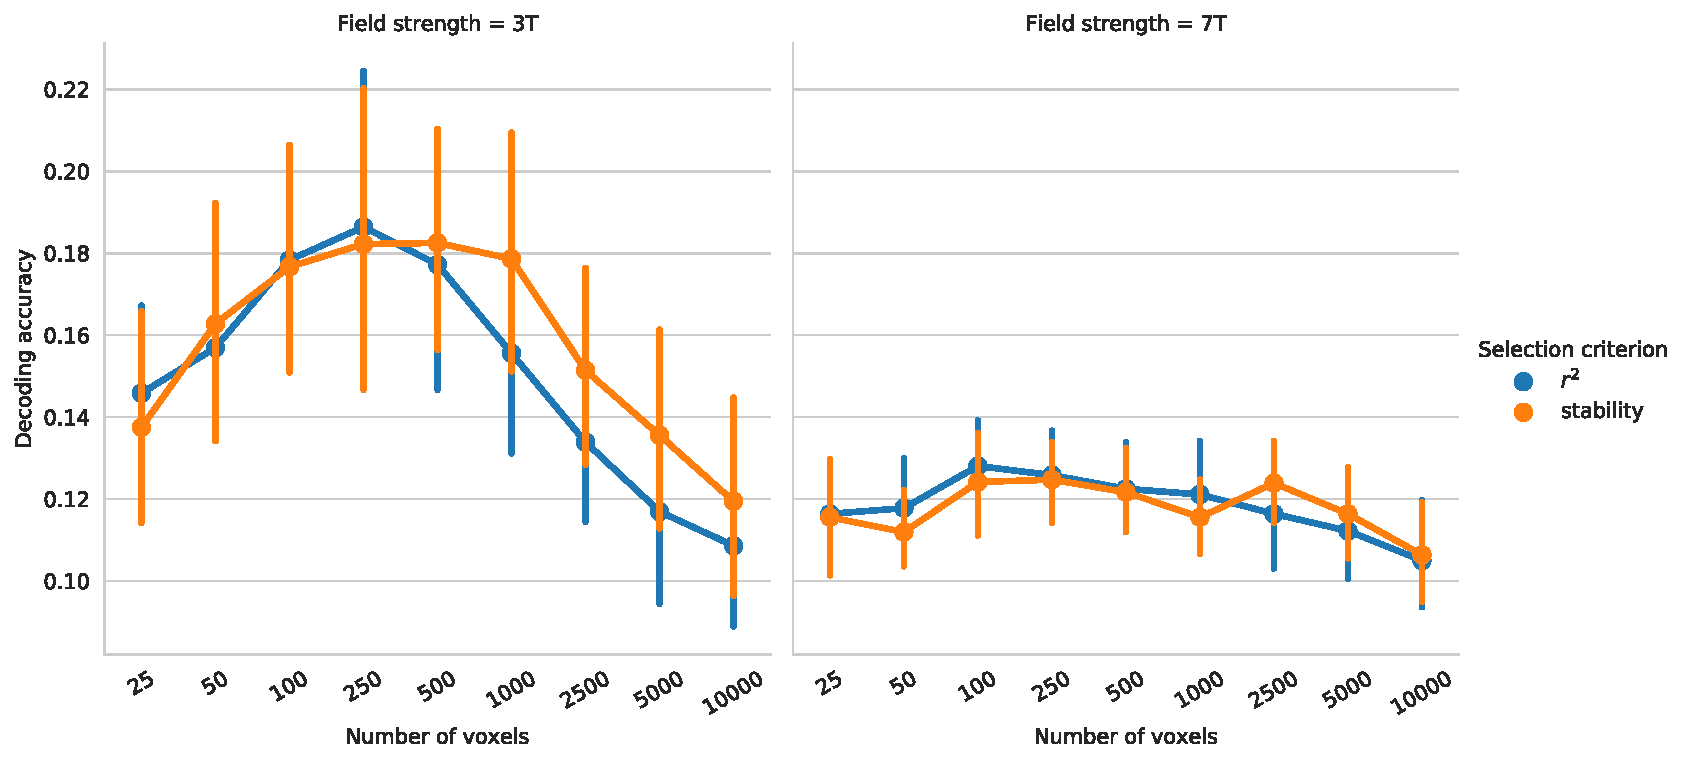
\includegraphics[width=\linewidth]{pics/decoding_selection.pdf}

	\caption{\textbf{A} Mean decoding accuracy of individual music stimuli as a function of
  the included number of voxels for 3T and 7T, for stability- and
  $r^2$-based voxel selection. Error bars denote the bootstrapped 95\%
  confidence interval of the mean. The mean is taken over decoding
  accuracies of eight runs for each of the 19 participants. Chance level is
    0.04. \textbf{B} Mean
decoding accuracy of individual music stimuli as a function of the overall volume of the
included voxels for 3T and 7T, for stability- and $r^2$-based voxel
selection. Chance level is 0.04.
}
 \label{fig:decoding_accuracy_stimulus_selection}
\end{figure}

\begin{figure}
  \centering
  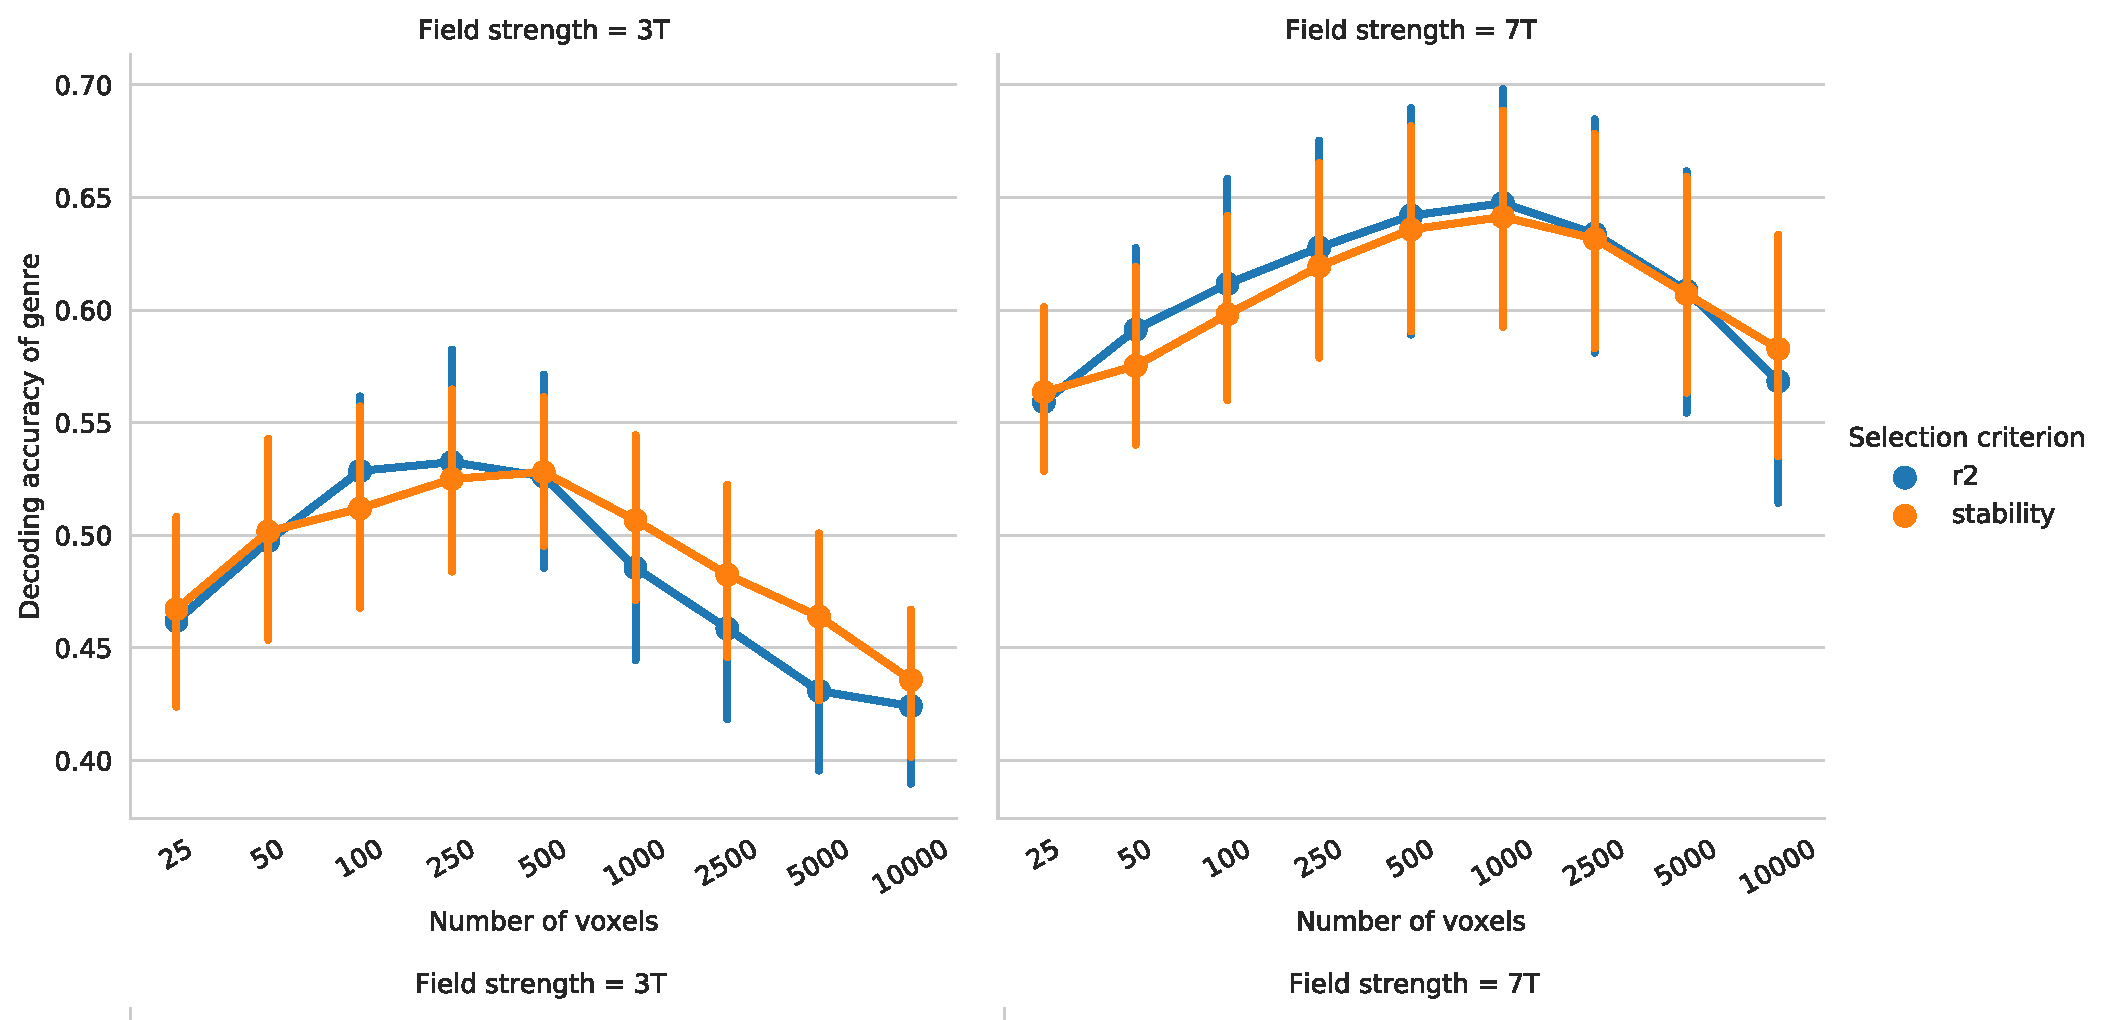
\includegraphics[width=\linewidth]{pics/decoding_genre_selection.pdf}

  \caption{\textbf{A} Mean decoding accuracy of music category as a function of
  the included number of voxels for 3T and 7T, for stability- and
  $r^2$-based voxel selection. Error bars denote the bootstrapped 95\%
  confidence interval of the mean. The mean is taken over decoding
  accuracies of eight runs for each of the 19 participants. \textbf{B} Mean
decoding accuracy of music category as a function of the overall volume of the
included voxels for 3T and 7T, for stability- and $r^2$-based voxel
selection.
}

 \label{fig:decoding_accuracy_selection}
\end{figure}



\end{document}

% vim: textwidth=80 colorcolumn=81
